\chapter{Analyse der AGN Mrk 421}
\label{chapter:Analyse}

Im folgenden Kapitel werden die Gamma-Hadron-Separation und Energierekonstruktion (\autoref{sec:GH-Separation}), die Erstellung von Lichtkurven (\autoref{sec:Lichtkurve}) und die Spektrums-Rekonstruktion (\autoref{sec:Unfolding}) erläutert.
Zu diesem Zweck werden Standard\-/Analyseprogramme benutzt, die im \textit{MARS} (MAGIC Analysis and Reconstruction Software)-Paket enthalten sind.
Dieses Softwarepaket beinhaltet eine Sammlung von ROOT-Skripten und Macros \cite{MARS}, wie \textit{coach}, womit der Random Forest trainiert wird, \textit{flute}, womit die Lichtkurve bestimmt wird oder \textit{CombUnfold}, was der Entfaltung des Energiespektrums dient. 

Nach einer kurzen Einführung in diese Programme, werden diese in \autoref{Mrk421_Analyse} für die Analyse der 2012 aufgenommenen Daten der AGN Mrk~421 genutzt.
Der Datensatz des gesamten Jahres 2012 wird auf Grund von Änderungen der abbildenden Eigenschaften des Teleskops und Hardwareänderungen in vier Teile geteilt und einzeln analysiert. 
Für jeden Einzeldatensatz werden dedizierte MC-Daten benötigt.

In \autoref{LC_Alles} werden dann alle Ergebnisse zu einer gesamten Lichtkurve zusammengefasst und die ermittelten Spektren miteinander verglichen.


\section{Gamma-Hadron-Separation und Energieschätzung}
\label{sec:GH-Separation}
Im Folgenden wird ein Überblick über die Methode der Gamma-Hadron-Separation (GH-Separation), die Energieschätzung sowie die Rekonstruktion der Quellposition gegeben.  
Hierzu wird die Methode des Random-Forests erklärt, welcher zur Gamma-Hadron-Separation und zur Rekonstruktion der Quellposition genutzt wird.
Weiterhin wird die Benutzung von Look-Up-Tabellen erläutert, welche zum Schätzen der Energie eines Ereignisses genutzt wird.
%mit denen die Energie eines Ereignisses geschätzt wird.


\subsection{Gamma-Hadron-Separation}
Da das Signal-Untergrund-Verhältnis zwischen Gamma-Schauern aus Richtung der Quelle und hadronischen Schauern kleiner als 1:1000 ist, werden effiziente Verfahren benötigt, um das Signal vom Untergrund zu trennen.\cite{Bock}
Diese geringe Anzahl an Signalereignissen ist sogar für helle Quellen wie Crab vorhanden.
In der Standard-MAGIC-Analysekette übernehmen die Programme \textit{Coach} und \textit{Melibea} diese Aufgabe. 
Zu diesem Zweck wird ein Random Forest (RF) genutzt \cite{RandomForestForMAGIC}.
Dieser RF basiert auf einem Ensemble an Entscheidungsbäumen mit zufällig ausgewählten Parametern an ihren Knoten.
Um einen solchen RF zu trainieren, wird ein Trainingsdatensatz aus MCs und Untergrunddaten benötigt, von denen die Klassenzugehörigkeit (Signal oder Untergrund) bekannt ist.

Jedes Ereignis wird durch die in \autoref{sec:Star-ImageCleaning} beschriebenen Bildparameter charakterisiert.
Im Ausgangsknoten eines jeden Entscheidungsbaumes befindet sich der komplette Datensatz mit allen Bildparametern.
Dieser Knoten wird dann in zwei Nachfolgeknoten geteilt, indem in einem Bildparameter geschnitten wird.
Bei diesem Splittingprozess wird eine bestimmte Anzahl an Parametern für den Schnitt zufällig aus einer vorher begrenzten Menge gezogen und der Parameter mit dem minimalen Gini-Index zur Separation genutzt.\cite{RandomForestForMAGIC}

Mit Hilfe des Gini-Index' kann die Ungleichheit der beiden Verteilungen als Funktion des Schnittes angegeben werden.
Ist der Gini-Index von einem Knoten null, so ist in diesem Knoten nur noch eine Klasse vorhanden.\cite{RandomForestForMAGIC}
% So bedeutet ein kleiner Gini-Koeffizient, dass die Verteilungen ähnlich sind und ein großer, dass sie ungleich sind. 

Weitere Schnitte werden so lange durchgeführt bis die Anzahl der Ereignisse in einem Knoten zu gering wird oder in einem Knoten nur noch eine Klasse vertreten ist.
In diesen Endknoten (Terminal Nodes) werden die Ereignisse mit einem Label $l_i$ (Gamma oder Hadron) versehen. 
%Befindet sich in einem Endknoten noch eine Mischung beider Klassen, wird ein Mittelwert vergeben.
Dieser Prozess wird anschließend für alle weiteren $i$ Entscheidungsbäume durchgeführt bis der Random Forest vollständig gebildet wurde.\cite{RandomForestForMAGIC}

Beim Anwenden des RF folgt jedes Ereignis einem Pfad durch die $i$ verschiedenen Bäume und wird von allen klassifiziert.
Danach wird jedem Ereignis eine Hadroness $h$ als finaler Wert zugewiesen, der die Wahrscheinlichkeit angibt, dass das Ereignis ein Hadron ist.
Dies geschieht durch der Entscheidungen aller Bäume \cite{RandomForestForMAGIC}: 

\begin{equation}
 h(Ereignis)=\frac{ \sum_{i=1} ^{n_{B\ddot{a}ume}} l_i(Ereignis)}{n_{B\ddot{a}ume}}.
\end{equation}

Es ist möglich in dem Programm \textit{Coach} alle Parameter auszuwählen, die zum Training des RFs für die GH-Separation verwendet werden.
Die Parameter für die \texttt{Disp}-Bestimmung sowie zum Bauen der Look-Up-Tables zur Energierekonstruktion werden ebenfalls in \textit{Coach} ausgewählt.
Bei der GH-Separation werden in dieser Analyse elf verschiedene Parameter wie zum Beispiel \texttt{Width} oder \texttt{Length} genutzt.
Des Weiteren ist es möglich die Anzahl der Bäume, sowie die Anzahl der gezogenen Parameter auszuwählen mit denen der RF trainiert werden soll.

\subsection{Energierekonstruktion mit Hilfe von Look-Up-Tables}
Die Energie der Primärteilchen ist proportional zur Anzahl der Cherenkov-Photonen im Schauer und somit auch zum Parameter \texttt{size}.
Allerdings ist \texttt{size} abhängig vom Zenitwinkel, der Lage des Schauers in der Kamera, dem Impact-Parameter und der Höhe des Schauermaximums.\cite{EnergieRekonstruktion}

Aufgrund dieser Abhängigkeiten wird eine Tabelle erstellt.
Der MC\-/Trainingsdatensatz wird in Bins für jeden Parameter, der für die Energierekonstruktion benutzt werden soll, aufgeteilt.
%So wird eine mehrdimensionale Tabelle mit der gemittelten Energie der MC-Ereignisse, die zu jedem Bin gehört, erstellt.
Anschließend wird in dieser mehrdimensionalen Tabelle in jedem Bin über die MC-Energien gemittelt sowie der quadratische Mittelwert bestimmt, sodass jedem Bin in dieser Tabelle eine Energie zugeordnet ist.
Einem realen Ereignis wird anhand seiner Parameter das passende Energie-Bin in der Tabelle zugeteilt und so eine geschätzte Energie (\texttt{Estimated Energy}) zugewiesen.
Für eine genauere Energierekonstruktion werden noch einige Korrekuren angewandt.
Schauer, die nicht vollständig in der Kamera enthalten sind, bedürfen beispielsweise solch einer Korrektur.\cite{EnergieRekonstruktion}

Für Mono-Daten geschieht die Energierekonstruktion mit Hilfe einer Random Forest Regression.
Dieser Algoritjmus schätzt keine Klassenzugehörigkeit von Ereignissen, sondern den Wert einer kontinuierlichen Funkion. 
In diesem Fall ist der Wert ein Energieschätzer.
Um den finalen Wert zu bestimmen, wird nach der Anwendung aller Bäume über die Ergebnisse der einzelnen Bäume gemittelt.\cite{EnergieRekonstruktion} 


\subsection{Rekonstruktion der Quellposition}
In diesem Abschnitt wird die Bestimmung des Parmeters \texttt{Disp} beschrieben, mit Hilfe dessen die Herkunft des Primärteilchens rekonstruieren werden kann. 
Der Parameter \texttt{Disp} bezeichnet den Abstand zwischen dem Schauerschwerpunkt und der Quellposition in der Kamera.
Für Beobachtungen mit nur einem Teleskop gibt es zwei Möglichkeiten, diesen Parameter zu rekonstruieren. 
Zum Einen sind dies sogenannte Ghost-Busting-Methoden, die die Asymmetrie des Schauers charakterisieren und zum Anderen eine Random Forest Regression.\cite{DispRekonstruktion}

Bei den Ghost-Busting-Methoden werden Parameter genutzt, die die Asymmetrie zwischen Schaueranfang und Schauerende in der Kamera charakterisieren.
%Mit Hilfe des zeitlichen Verlaufs oder des dritten Moments entlang der Hauptachse wird entschieden, aus welcher Richtung der Schauer kommt.
Mit Hilfe von Zeitgradienten der Ankunftszeiten oder des dritten Moments der Verteilung entlang der großen Halbachse wird entschieden aus welcher Richtung der Schauer kommt.\cite{DispRekonstruktion}

In einer Standardanalyse geschieht die Rekonstruktion des Parameters \texttt{Disp} für ein Teleskop mit einer Random Forest Regresssion.
Wie in \autoref{Disp} zu sehen ist, sind zwei Positionen für den Parameter \texttt{Disp} wahrscheinlich.
Diese befinden sich auf der Schauerachse in den gleichen Entfernungen vom Schauerschwerpunkt.
Durch Mittelung über die Ergebnisse der Bäume wird der wahrscheinlichere Wert bestimmt.\cite{DispRekonstruktion}

Wird mit zwei Teleskopen observiert, ist die \texttt{Disp}-Rekonstruktion einfacher als mit einem Teleskop.
Das Vorgehen dabei besteht aus zwei Schritten.
Zunächst werden mit Hilfe einer Random Forest Regression die zwei möglichen \texttt{Disp}-Werte bestimmt.
Mit diesen Werten ist dann wie in \autoref{Disp} zu sehen ist, eine effiziente Bestimmung der tatsächlichen Quellposition möglich.

\begin{figure}
    \centering
    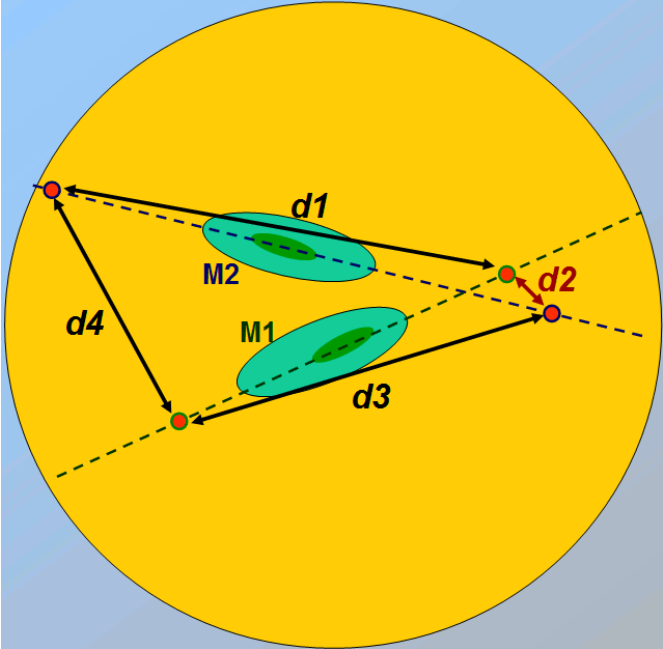
\includegraphics[width=0.5\textwidth]{./Plots/04_MrkAnalyse/Disp.png}
    \caption{Schema zur Rekonstruktion des Stereo-Parameters \texttt{Disp}. 
    Dargestellt sind die aufgenommenen Schauer beider Kameras, projiziert auf eine Kameraebene.
    Die roten Punkte stellen die möglichen Quellpositionen des Schauers in der Kamera von MAGIC-I (im Bild: M1) und MAGIC-II (im Bild: M2) dar.
    Die Abstände zwischen den rekonstruierten Quellpositionen der beiden Teleskope werden durch $d_i$ dargestellt. 
    Der kleinste Wert für $d_i$ beschreibt hier den Abstand zwischen den beiden wahrscheinlicheren \texttt{Disp} -Werten.
    Aus den Abständen dieser Punkte zueinander kann entschieden werden, welche Herkunftsrichtung für den Schauer am wahrscheinlichsten ist.\cite{DispRekonstruktion}}
    \label{Disp}
\end{figure}

Nur eine der beiden möglichen Quellpositionen des einen Teleskops ist kompatibel mit einer der rekonstruierten Quellpositionen des anderen Teleskops. 
Die bevorzugte Position der Quelle ist die, die näher am Schnittpunkt der beiden Hauptachsen liegt und bestimmt \texttt{Disp} für beide Teleskope eindeutig.
Letztendlich wird der mit dem Abstand zum Schnittpunkt der Hauptachsen gewichtete Mittelwert der beiden wahrscheinlichsten rekonstruierten Quellpositionen gewählt.
Ereignisse mit einer zu großen Differenz der beiden rekonstruierten Quellpositionen zueinander werden bei der GH-Separation verworfen.\cite{DispRekonstruktion}


\section{Berechnung der Lichtkurve}
\label{sec:Lichtkurve}
Die zeitliche Entwicklung des integralen Flusses der Gammastrahlung wird als Lichtkurve bezeichnet.
Die Rate der Gammaphotonen pro Einheitsfläche und Zeit ist die Ausgangsgröße für die Lichtkurve:

\begin{equation}
 \Phi=\frac{\mathrm{d}^2 N}{\mathrm{d}S \, \mathrm{d}t} 
\end{equation}

 \begin{center}
  \small{mit $N$: Anzahl der Teilchen, $S$: Fläche und $t$: Zeit.}
 \end{center}
 
Zur Bestimmung des Flusses werden die Anzahl der detektierten Gammas, die effektive Observationszeit und die effektive Fläche des Detektors benötigt.
%Nach der Energie differenziert ist diese Größe der differentielle Fluss pro Energie:
Wird diese Größe nach der Energie differenziert, stellt die Größe $\frac{\mathrm{d}\Phi}{\mathrm{d}E}$ den differentiellen Fluss pro Energie dar:

\begin{equation}
 \frac{\mathrm{d}\Phi}{\mathrm{d}E}=\frac{\mathrm{d}^3N}{\mathrm{d}S \, \mathrm{d}t \, \mathrm{d}E}.
\end{equation}

Der integrale Fluss oberhalb einer bestimmten Energieschwelle (z.B. \SI{500}{GeV}) kann anschließend mit:

\begin{equation}
 \Phi_{E>500GeV}=\int\limits_{\SI{500}{GeV}}^{\infty}\frac{\mathrm{d}\Phi}{\mathrm{d}E}\mathrm{d}E
\end{equation}

berechnet werden.
Trägt man diese Größe gegen die Zeit auf, erhält man die Lichtkurve.\cite{Lichtkurve}

% Das Binning muss dabei so gewählt werden, dass die Statistik in jedem Bin groß genug ist.
% , tageweise oder minutenweise... Je nachdem, ob gerade irgendwas spannendes passiert (Flares oder so).

\paragraph{Anzahl der Signalereignisse}
Um die Anzahl der Signalereignisse, d.h. Gammaphotonen aus der Quelle zu bestimmen, wird ein $\theta^2$-Histogramm benutzt.
Dies ist ein Histogramm der quadrierten Entfernungen zwischen der rekonstruierten Quellposition und der nominalen Quellposition.
Gammaphotonen aus der Quelle haben ein kleineres $\theta$, während der Background eine annähernd isotrope Verteilung liefert. 
%Dies ist beispielhaft in \autoref{Crab_Theta2} gezeigt: schwarz ist die Verteilung der Signal-Ereignisse rot ist die Verteilung der Background-Ereignisse und blau die Differenz aus Signal und Background-Ereignissen. 
Dieses Verhalten ist exemplarisch in \autoref{Crab_Theta2} für On-, Off- und Signalereignisse dargestellt.

\begin{figure}
    \centering
    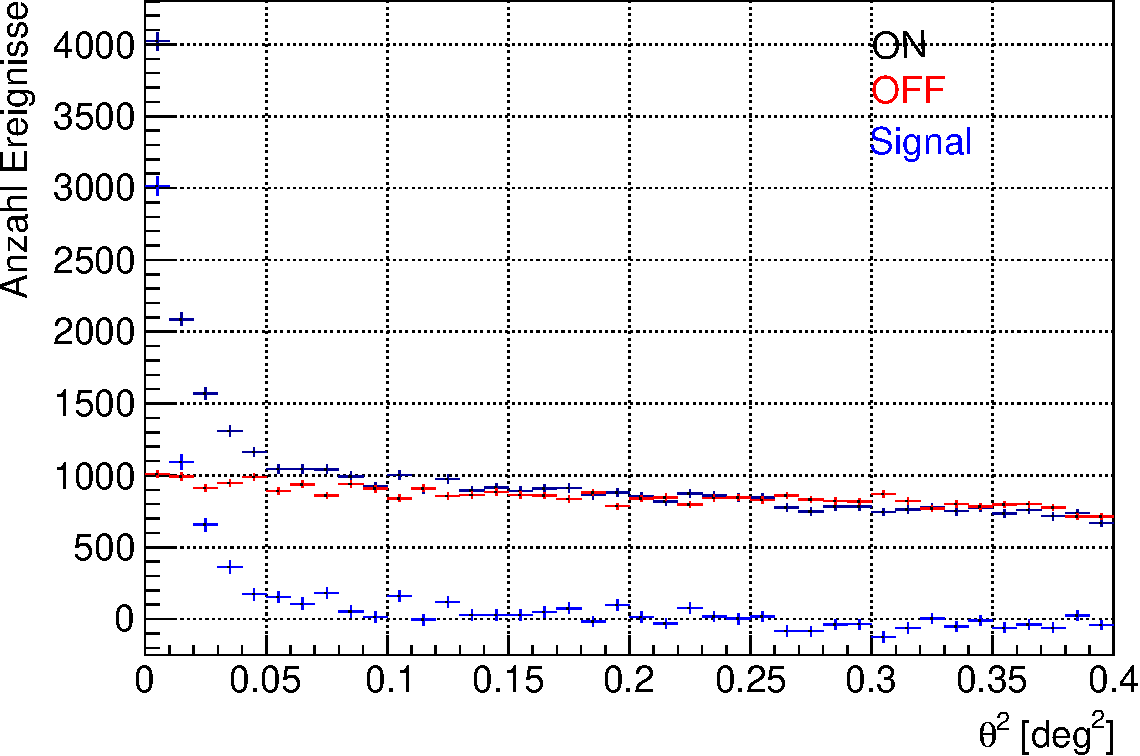
\includegraphics[width=0.8\textwidth]{./Plots/04_MrkAnalyse/Datenset2/Crab_Theta2.pdf}
    \caption{$\theta^2$-Verteilung von Crab-Daten aus dem Datensatz 2. 
    Es ist zu sehen, dass die On- (schwarz) und die Off-Daten (rot) für $\theta^2 > 0,1$ miteinander übereinstimmen.
    Des Weiteren werden die Signal-Daten in blau dargestellt, die sich aus den On-Daten nach Subtraktion der Off-Daten ergeben.
    Ereignisse aus der Quelle befinden sich wie erwartet bei $\theta^2 \approx 0$.
    }
    \label{Crab_Theta2}
\end{figure}
% BILDBILDBILD (abelardos talk in zeuthen, der auf der flute seite verlinkt ist)

Um die Anzahl der realen Signal-Ereignisse zu ermitteln, müssen von den Ereignissen aus der Quellrichtung noch die Background Ereignisse subtrahiert und ein Schnitt in $\theta^2$ angewendet werden.

Dank der ``Wobble-Beobachtung`` ist eine simultane Datennahme von Signal- und Hintergrund möglich.
Bei dieser Beobachtungsmethode ist das Teleskop nicht direkt auf die Quelle ausgerichtet, sondern die Quellposition ist $0.4°$ vom Kamerazentrum entfernt.
Wegen der Alt-Azimutalen Montierung rotiert die Quelle um das Zentrum in der Kamera und es ist möglich einen Punkt gegenüber der Quelle als Off-Position zu benutzen.
%Vorteil dieser Methode ist, dass es keine separate Off-Datennahme geben muss.
Es muss gewährleistet werden, dass die Off-Positionen symmetrisch verteilt sind, um Kamerainhomogenitäten entgegenzuwirken.
Allerdings tauchen bei dieser Methode die Photonen aus der Quelle auch in der Off-$\theta^2$-Verteilung auf, haben aber ein großes $\theta^2$.
Eine Off-Position, die zu nahe an der Quelle ist, ist aufgrund der beschriebenen Nachteile ungünstig.\cite{Lichtkurve}

\paragraph{Effektive Beobachtungszeit}
Die effektive Beobachtungszeit berücksichtigt die Totzeit in der Datennahme.
Nach dem Aufnehmen eines Ereignisses ist die Elektronik mit der Verarbeitung der Daten beschäftigt und neue Ereignisse können nicht detektiert werden.
Die Totzeit ist abhängig vom Chip und beträgt bei den aktuellen DRS4-Chips einige $\mu s$.\cite{Lichtkurve}

\paragraph{Effektive Fläche}
Als effektive Fläche wird die Fläche auf Teleskophöhe bezeichnet, die orthogonal zur Herkunftsrichtung der Schauerteilchen ist.
Die Größe dieser effektiven Fläche ist abhängig von der Energie und dem Zenitwinkel des Schauers, sowie von Analyseschnitten.
In \textit{MARS} wird diese Größe mit Hilfe von MCs folgendermaßen berechnet:

\begin{equation}
 A_{eff}(E)=\frac{N_{\gamma, final}}{N_{\gamma, simulated}}A_{MC, total}
\end{equation}

Dafür wird eine bestimmte Anzahl an simulierten Gammaphotonen ($N_{\gamma, simulated}$) auf einer uniformen Fläche $A_{MC,total}$ simuliert. 
Die Größe $N_{\gamma, final}$ drückt die Anzahl der Gammaphotonen aus, die alle Analyseschnitte überlebt haben.\cite{Lichtkurve}


\section{Entfaltung des Energiespektrums}
\label{sec:Unfolding}
Bei der Messung mit IACTs handelt es sich um eine indirekte Messung.
Die Energie des Schauer-auslösenden Teilchens ist nicht direkt messbar.
Die Bildparameter und damit auch die geschätzte Energie $E_{est}$ haben eine begrenzte Auflösung und erfordern die Methode der Entfaltung.

Die Probleme bei der Messung lassen sich wie folgt zusammenfassen \cite{UnfoldingTheorie}:

\begin{itemize}
 \item Begrenzte Akzeptanz: Nicht alle Schauer, die Teilchen auslösen, können vom Teleskop detektiert werden.
 \item Indirekte Messung: Da eine direkte Messung nicht möglich ist, wird anhand von gemessenen Parametern, wie z.B. der Größe des Schauers in der Kamera, mit Hilfe eines RF die Energie geschätzt.
       Die Vorraussetzung dafür ist, dass diese real gemessenen Parameter stark mit der Energie korrelliert sind.
 \item Begrenzte Auflösung: Es ist nur möglich mit begrenzter Genauigkeit aus den Bildparametern die Energie zu rekonstruieren, d.h. es existiert eine Migration von Ereignissen.
       Wird die geschätzte Energie gegen die reale Energie aufgetragen, erhält man eine verschmierte Diagonale (siehe Abb.\ref{EnergyEst_EnergyTrue})
\end{itemize}

\begin{figure}
    \centering
    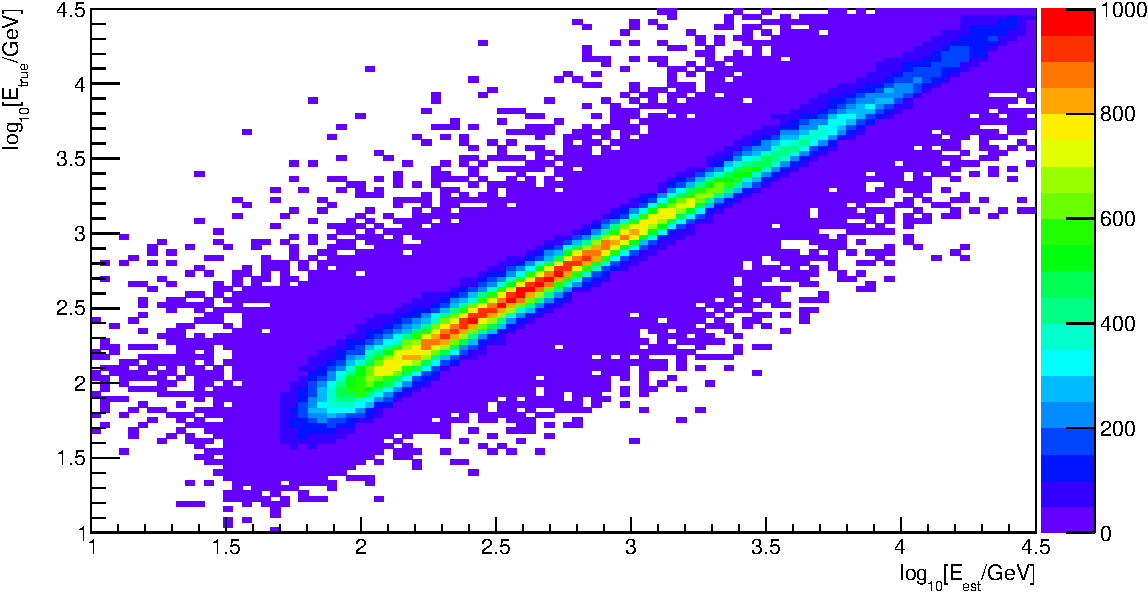
\includegraphics[width=0.8\textwidth]{./Plots/04_MrkAnalyse/EnergyEst_EnergyTrue.pdf}
    \caption{Dargestellt ist ein zweidimensionales Histogramm, in dem die geschätzte Energie gegen die wahre Energie aufgetragen ist. 
    Es ist erkennbar, dass keine perfekte Energierekonstruktion existiert.}
    \label{EnergyEst_EnergyTrue}
\end{figure}

Durch die Methode der Entfaltung können diese Probleme berücksichtigt werden. 
Das Problem lässt sich mit einer Fredholmschen Integralgleichung darstellen \cite{Blobel}:

\begin{equation}
 g(y)= \int\limits_c^d M(x,y) f(x) \mathrm{d}x + b(y)
\end{equation}
\begin{center}
  \small{mit $g(y)$: gemessene Verteilung, $f(x)$: gesuchte Verteilung, $M(x,y)$: Migrationsmatrix bestimmt auf MCs, $b(y)$: Background-Verteilung}
 \end{center}

Diese Gleichung lässt sich diskretisieren zu:

\begin{equation}
 g_i=\sum_j M_{ij}f_j+b_i,
\end{equation}

wobei $M_{ij}$ die Migrationsmatrix ist und damit die Wahrscheinlichkeit beschreibt, dass ein Ereignis in bin $j$ zum Energiebin $i$ zugeordnet wird.

Das Ziel der Entfaltung ist die wahre Verteilung $f$ zu finden.
Die Kovarianzmatrix der gesuchten Verteilung ergibt sich mit der Kovarianzmatrix der gemessenen Verteilung zu:

\begin{equation}
 \mathbf{V[\vec{f}]}=\mathbf{M}^{-1}\mathbf{V}[\vec{g}]\mathbf{(M}^{-1})^T.
\end{equation}

Da die Invertierung der Migrationsmatrix oft zu oszillierenden Lösungen führt, wird die Methode der kleinsten Quadrate angewandt.

\begin{equation}
 \chi_0^2=(\vec{g}-\mathbf{M}\vec{f})^T \mathbf{V}^{-1}[\vec{g}](\vec{g}-\mathbf{M}\vec{f}).
\end{equation}

% Dies gilt nur für Gauß-verteilte Daten, also nicht für Bins mit kleinen Ereigniszahlen.
% Für diese muss nun die Poisson-Statistik benutzt werden und der Log-Likelihood-Ausdruck minimiert werden:
% 
% \begin{equation}
%  L_0(a)=\sum_i (g_i(a)-g_{i,m}\cdot \ln g_i(a)).
% \end{equation}

Außerdem ist es nötig, eine Regularisierung einzuführen, um die kleinen Ausdrücke in der Migrationsmatrix, die während der Entfaltung verstärkt werden, zu unterdrücken.
Durch Einführung eines Regularisierungsterms werden Anforderungen an die Lösung gestellt.
Bei zu starker Regularisierung führt dies allerdings zu einem Bias hin zum Trainingsspektrum.

Im Allgemeinen wird Regularisierung durch Addition eines Regularisierungsterms berücksichtigt und lässt sich darstellen als:

\begin{equation}
 \chi^2=\frac{\tau}{2}\chi_0^2 + Reg(f).
\end{equation}

Verschiedene Arten der Regularisierung können in der Analyse gewählt werden.\cite{CombUnfold}

Es ist auch möglich, eine Vorwärtsfaltung durchzuführen, wobei ein bestimmtes Modell als Annahme gewählt wird und freie Parameter dieses Modells bestimmt werden.\cite{CombUnfold}
Zum Testen ist dies eine gute Alternative, allerdings keine richtige Entfaltung, da das Ergebnis modellabhängig bleibt und physikalische Phänomene verborgen bleiben.

\section{Mrk 421-Analyse}
\label{Mrk421_Analyse}
In diesem Abschnitt wird die Analyse der Daten beschrieben, wobei für jede der vier Datenepochen sowohl die Lichtkurve als auch das Spektrum gezeigt werden.
Dabei wird die Analyse des Datensets 2 der Daten exemplarisch für die Stereo-Analyse erklärt (\autoref{subsec:Datenset_2}), während die anderen Zeitabschnitte des Jahres mit stereoskopischer Beobachtung (\autoref{subsec:Datenset_1} und \autoref{subsec:Datenset_4}) analog ausgewertet werden.
Auf die Mono-Datenanalyse wird in \autoref{subsec:Datenset_3} eingegangen.
Zusammenfassend wird noch eine Lichtkurve aller Daten gezeigt.


\subsection{Überblick über die Daten}
Die Daten, die für diese Analyse zur Verfügung standen, sind Daten der Quelle Mrk~421, die 2012 aufgenommen wurden.
Die Daten gliedern sich folgendermaßen:

\begin{itemize}
 \item Datenset 1: 2012-02-25 - 2012-02-29
 \item Datenset 2: 2012-03-18 - 2012-04-27
 \item Datenset 3: 2012-05-23 - 2012-06-19 (Mono)
 \item Datenset 4: 2012-12-11 - 2012-12-23
\end{itemize}

Datenset 1 und Datenset 2 sind Stereobeobachtungen.
Die beiden Datensets unterscheiden sich in ihrer PSF (Point Spread Function), weswegen zwei verschiedene MC-Sets in der Analyse verwendet werden.
Die PSF beschreibt die Abbildungsqualität der Spiegel, bzw. wie gut diese ausgerichtet sind.
Je größer die PSF ist, desto schlechter sind die Abbildungseigenschaften und umso verschmierter ist die Reflexion einer Punktquelle.

Beim Datenset 3 handelt es sich um Mono-Daten. 
Aufgrund der defekten MAGIC-I-Kamera und der geplanten Upgrade-Pause, wurde nur MAGIC-II betrieben.

Im Datenset 4 war das Upgrade abgeschlossen, die alte MAGIC-I-Kamera durch eine neue Kamera ersetzt und es wurden wieder Stereo-Beobachtungen durchgeführt.
Aufgrund der Hardware-Veränderungen und einer anderen PSF wurde es hier nötig wieder neue MCs zu produzieren.

Die Analyse des zweiten Datensets befindet wird in \autoref{subsec:Datenset_2} und die des ersten Datensets in \autoref{subsec:Datenset_1} beschrieben.
Danach erfolgt die dritte Analyseperiode mit Stereobeobachtungen (Datenset 4) in \autoref{subsec:Datenset_4}.
Die Mono-Analyse wird abschließend in \autoref{subsec:Datenset_3} beschrieben.


\subsection{Datenset 2}
\label{subsec:Datenset_2}
Anhand der genommenen Mrk 421-Daten, zehn Tage zwischen dem 18.3.2012 (MJD: 56004.1) und dem 27.4.2012 (MJD: 56042.0), wird nun die Stereo-Analyse erklärt.

Diese Daten wurden in einem Zenitwinkelbereich zwischen 12° und 30° genommen (siehe Abb.\ref{Datenset2_fZD}).

\begin{figure}
    \centering
    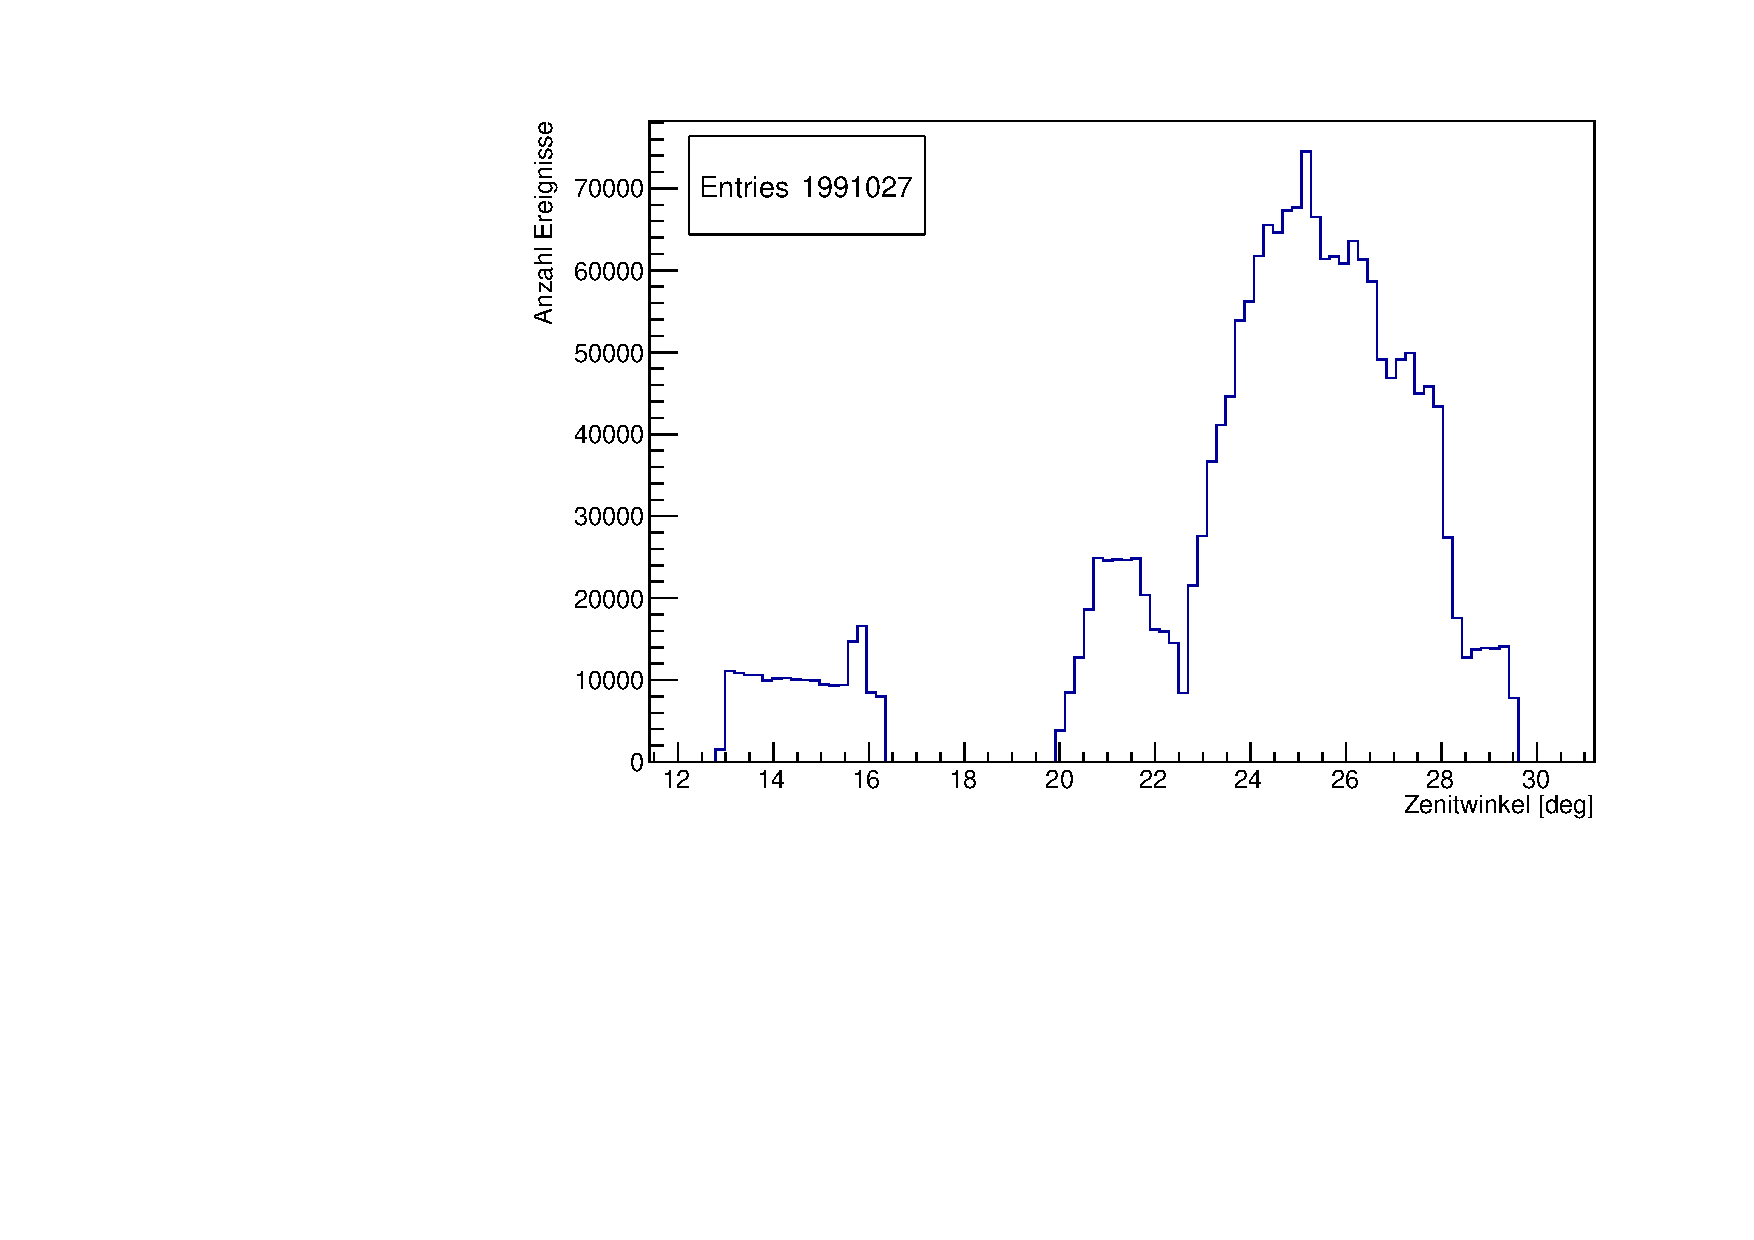
\includegraphics[width=0.7\textwidth]{./Plots/04_MrkAnalyse/Datenset2/Datenset2_Mrk421_MPointingPos_fZd.pdf}
    \caption{Zenitverteilung der genommenen Mrk 421-Daten zwischen dem 18.3.2012 und dem 27.4.2012.}
    \label{Datenset2_fZD}
\end{figure}


Da dieser Datensatz die meisten Daten beinhaltet, wird die Analyse exemplarisch hiermit durchgeführt.
Als Background-Daten dienen Daten anderer Quellen, welche in der gleichen Zeitspanne wie die zu analysierenden Daten liegen.
Dadurch wird gewährleistet, dass das Teleskop die gleichen Eigenschaften, wie z.B. PSF, hat wie bei der Datennahme der zu analysierenden Quelle. 
Mit Hilfe von Crab-Daten werden die Einstellungen für die Lichtkurvenbestimmung bestimmt, da Crab als Standardkerze dient und einen bekannten stabilen Fluss hat. 


\subsubsection{Daten-Auswahl und Qualitätchecks}
Zunächst werden die auf \textit{Superstar}-Level prozessierten Daten einem Datencheck unterzogen, um die Daten herauszufiltern, die bei guten Bedingungen genommen wurden.
Gute Bedingungen sind durch dunkle Nächte, gutes Wetter, wenig Störlicht durch z.B. Autoscheinwerfer und keine Hardware- oder Softwareprobleme gekennzeichnet.

Um dunkle Bedingungen zu gewährleisten wurde zunächst ein Cut im Direct Current (DC) (MAGIC-I < $\SI{500}{nA}$, MAGIC-II < $\SI{800}{nA}$) durchgeführt.
Anschließend wurden mit Hilfe des \textit{MARS} Macros \textit{Quate} alle Daten mit einem Zenitwinkel < 35° ausgewählt, Runs mit einer Länge unter $\SI{10}{s}$ und Runs mit einer Abweichung des Pointings von \SI{15}{arcmin} verworfen.
Außerdem wurden die Mittelwerte der Rate, der Parameter \texttt{Number of Islands}, \texttt{Concentration}, \texttt{Width} und \texttt{Length} gebildet und ebenfalls Ausreißer aussortiert, um eine gute Qualität der Daten zu gewährleisten.

Diese Kriterien für den Datencheck wurden für die Mrk 421-Daten, die Crab-Daten und die Background-Daten angewendet.

In der Tabelle \ref{tab:Datenset2-Mrk421} ist aufgelistet, an welchen Tagen Mrk 421-Daten nach dem Datencheck für die Analyse zur Verfügung stehen.


\begin{table}[!h]
\centering
\caption{Übersicht über alle nach dem Datencheck zur Verfügung stehenden Daten von Mrk~421 aus Datenset 2.}
\label{tab:Datenset2-Mrk421}
\begin{tabular}{ll}
  \toprule
  Monat & Tage\\
  \midrule
  \midrule
März & 18., 22., 28.\\
April & 11., 13., 15., 19., 21., 23., 25. \\
  \bottomrule
\end{tabular}
\end{table}

Tabelle \ref{tab:Datenset2} zeigt wieviele Minuten Daten, Background-Daten und Crab-Daten den Datencheck überstanden haben. 
Auf eine tageweise Auflistung der Background- und Crab-Daten wird an dieser Stelle verzichtet.

\begin{table}[!h]
\centering
\caption{Übersicht über alle an nach dem Datencheck zur Verfügung stehenden Daten von Mrk~421-, Crab- und Background aus Datenset 2.}
\label{tab:Datenset2}
\begin{tabular}{lc}
  \toprule
  Quelle & Observationszeit [min]\\
  \midrule
  \midrule
  Mrk 421 & 272\\
  \midrule
  Crab & 161\\
  \midrule
  0FGLJ0631 & 77 \\
  1ES1011 & 492 \\
  1ES1426 & 424 \\
  PG1553 & 971 \\
  PKS1222 & 247 \\
  SegueJ & 3252 \\
  \bottomrule
\end{tabular}
\end{table}

Für diesen Teil der Analyse werden die in Dortmund produzierten Standard-MC-Daten im Zenitbereich 5°-35° verwendet, in denen die alte MAGIC-I Kamera simuliert wurde.
Die PSF für MAGIC-I beträgt hierbei $\SI{10,5}{mm}$ und die Mirror Fraction 0.58, während diese Werte für MAGIC-II $\SI{10,2}{mm}$ für die PSF und 0.70 für die Mirror Fraction sind.

Es ist zu beachten, dass für alle Daten (Mrk 421/Crab/Background) und die MCs das gleiche Cleaning benutzt wird, da zu dieser Zeit zwei verschiedene Cleaning-Schwellen im Next-Neighbor-Cleaning gebräuchlich waren.
Die Schwellwerte für die Kern und Nachbarpixel betragen in diesen Daten 6, bzw. 3.


\subsubsection{\textit{Coach} und \textit{Melibea}}
Für das Training des RF für die GH-Separation und die \texttt{Disp}-Bestimmung sowie das Erstellen der Look-Up-Tables zur Energierekonstruktion ist es wichtig, dass in jedem Zenitbin ausreichend Background- und MC-Daten vorhanden sind.
Es wird ein Zenitbereich von 10-35° ausgewählt.
Wie in Abb.\ref{Datenset2_Zenitverteilung_Off} und Abb.\ref{Datenset2_Zenitverteilung_MC} zu sehen ist, ist diese Voraussetzung erfüllt.

\begin{figure}
    \centering
    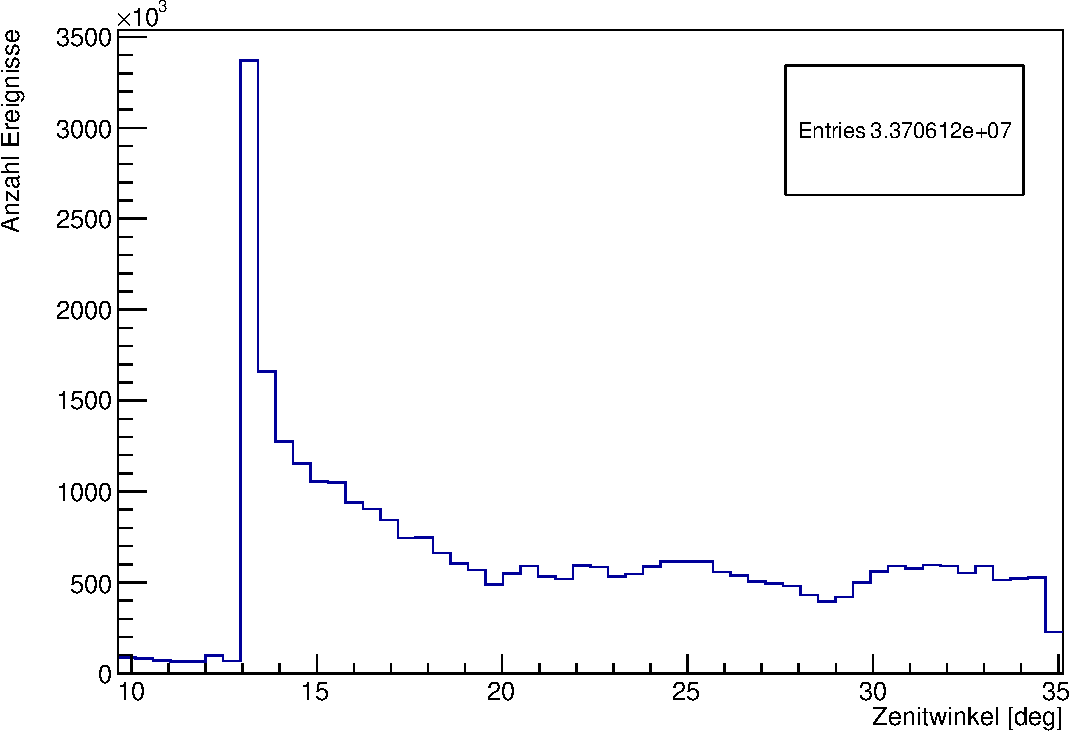
\includegraphics[width=0.7\textwidth]{./Plots/04_MrkAnalyse/Datenset2/Datenset2_Background_MPointingPos1_fZd.pdf}
    \caption{Zenitverteilung der Background-Daten zwischen dem 18.3.2012 und dem 27.4.2012.}
    \label{Datenset2_Zenitverteilung_Off}
\end{figure}

\begin{figure}
    \centering
    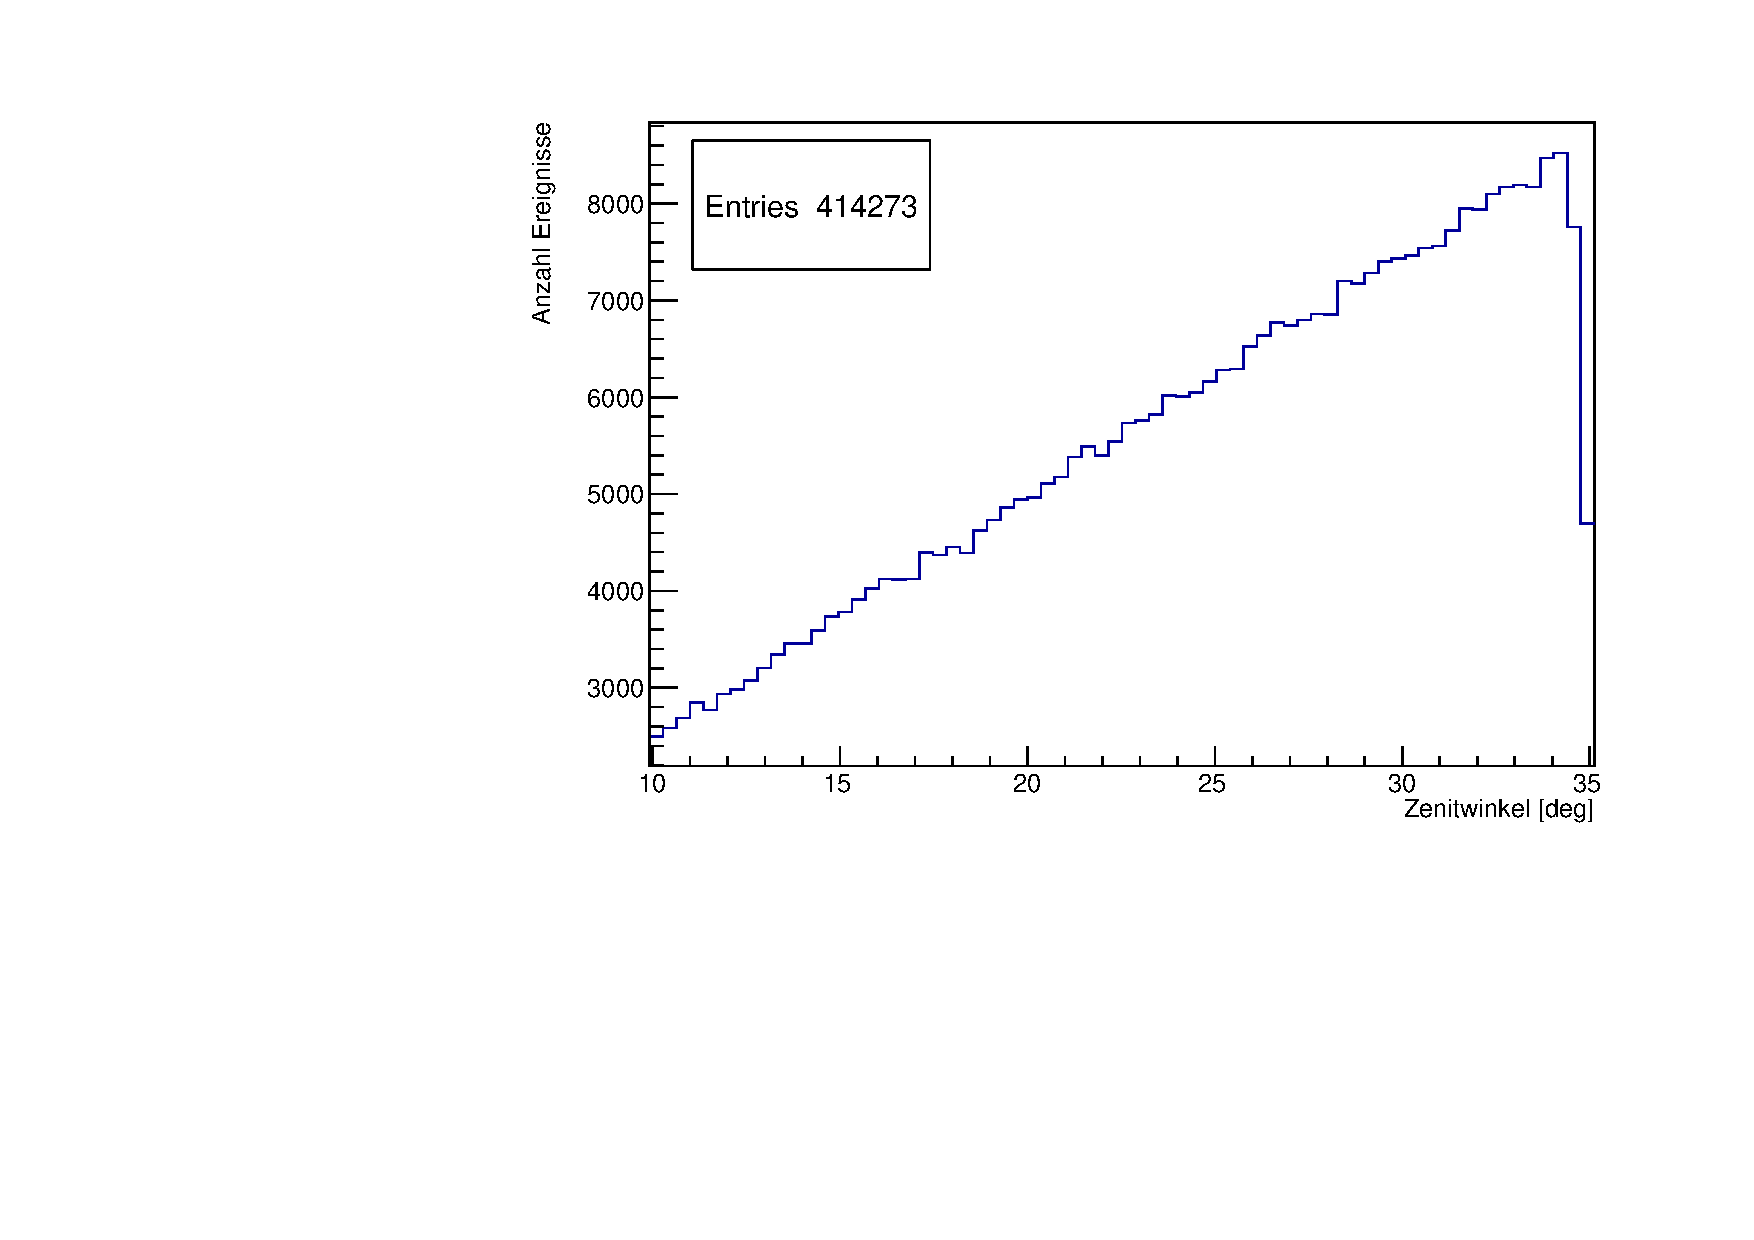
\includegraphics[width=0.7\textwidth]{./Plots/04_MrkAnalyse/Datenset2/Datenset2_MC_MPointingPos1_fZd.pdf}
    \caption{Zenitverteilung des Trainingssets der MC.}
    \label{Datenset2_Zenitverteilung_MC}
\end{figure}

Der MC-Datensatz wurde in zwei Teile geteilt.
Der eine Teil, das Trainings-Set, wird zusammen mit den Background-Daten zum Trainieren des RF für die GH-Separation und für die \texttt{Disp}-Abschätzung, sowie zum Aufstellen der Look-Up-Tables für die Energie benutzt.
Der andere Teil wird in nachfolgenden Analyseschritten zur Bestimmung der effektiven Fläche zur Entfaltung benutzt.

Sobald das Training der RFs und das Erstellen der Look-Up-Tables in \textit{Coach} beendet ist, werden in \textit{Melibea} die Daten nach Gamma- und Hadron-Ereignis klassifiziert und jedem Ereignis eine geschätzte Energie und ein \texttt{Disp}-Wert zugeordnet.
Das gleiche geschieht auch mit den Crab-Daten und dem anderen Teil der MCs, dem Test-Set.


\subsubsection{Lichtkurve: Crab}
Wie in \autoref{sec:Lichtkurve} beschrieben, wird nun sowohl für die Crab-Daten als auch für die Mrk 421-Daten eine Lichtkurve erstellt.
Da der Fluss von Crab stabil und bekannt ist, werden mit Hilfe der Crab-Daten die passenden Parameter (Hadroneffizienz und $\theta^2$-Effizienz) für die Lichtkurven-Bestimmung in diesem Zeitraum für Mrk~421 ausgewählt.

Wie in \autoref{Datenset2_Flute_Plots_Crab} zu sehen ist, ist es möglich mit \textit{Flute} neben der Lichtkurve (vgl. Abb.\ref{Datenset2_LC_Crab}) auch noch einen $\theta^2$-Plot (vgl. Abb.\ref{Datenset2_theta^2_Crab}), sowie die spektrale Energieverteilung (vgl. Abb.\ref{Datenset2_SED_Crab}) zu berechnen.

\begin{figure}
  %-----------------------------Figure 1--------------------------------------------------------%
  \begin{subfigure}{0.45\linewidth}
  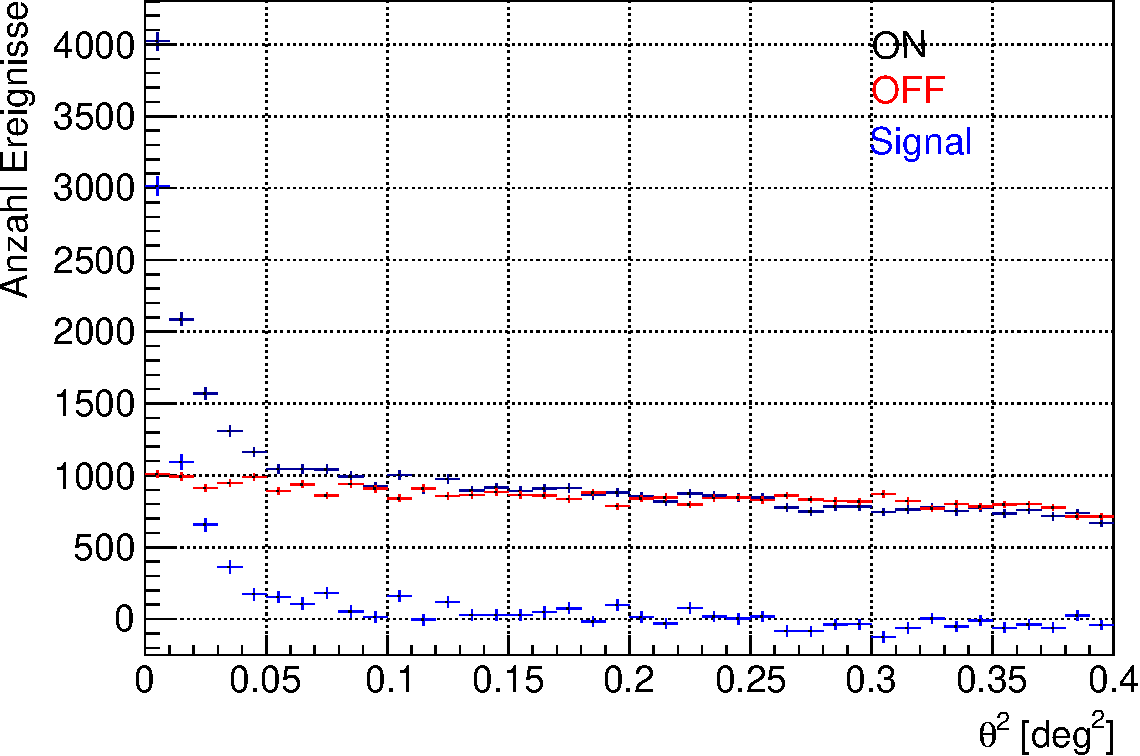
\includegraphics[width=\textwidth]{./Plots/04_MrkAnalyse/Datenset2/Crab_Theta2.pdf}
  \caption{$\theta^2$-Plot für Crab für alle Wobble-Positionen}
  %für den Energiebereich zwischen 5.5 GeV und 55.43TeV
  \label{Datenset2_theta^2_Crab}
  \end{subfigure}
  \hfill
  %-----------------------------Figure 2--------------------------------------------------------%
  \begin{subfigure}{0.45\linewidth}
  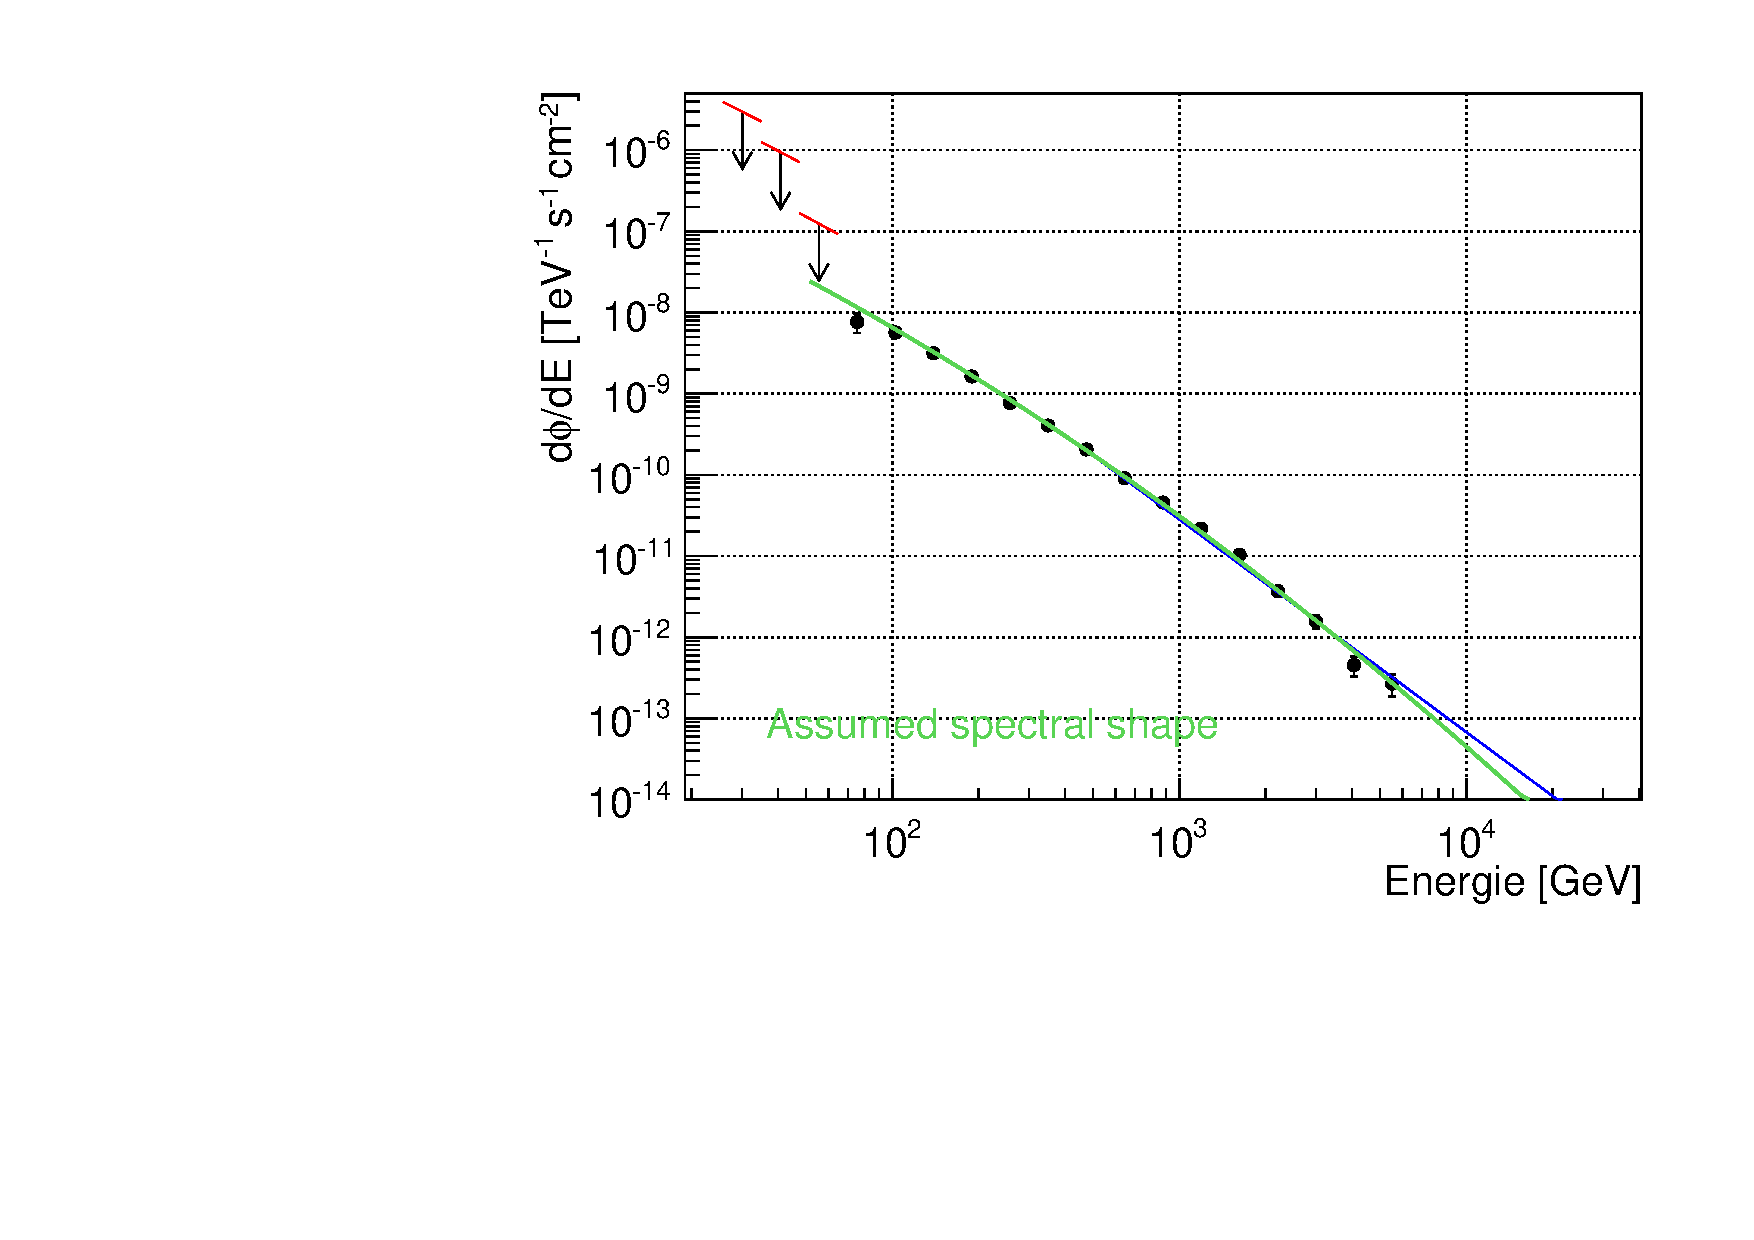
\includegraphics[width=\textwidth]{./Plots/04_MrkAnalyse/Datenset2/Crab_dFdE.pdf}
  \caption{Differentielles Energiespektrum}
  \label{Datenset2_SpectralShape_Crab}
  \end{subfigure}
  \hfill
  %-----------------------------Figure 3--------------------------------------------------------%
  \begin{subfigure}{0.45\linewidth}
  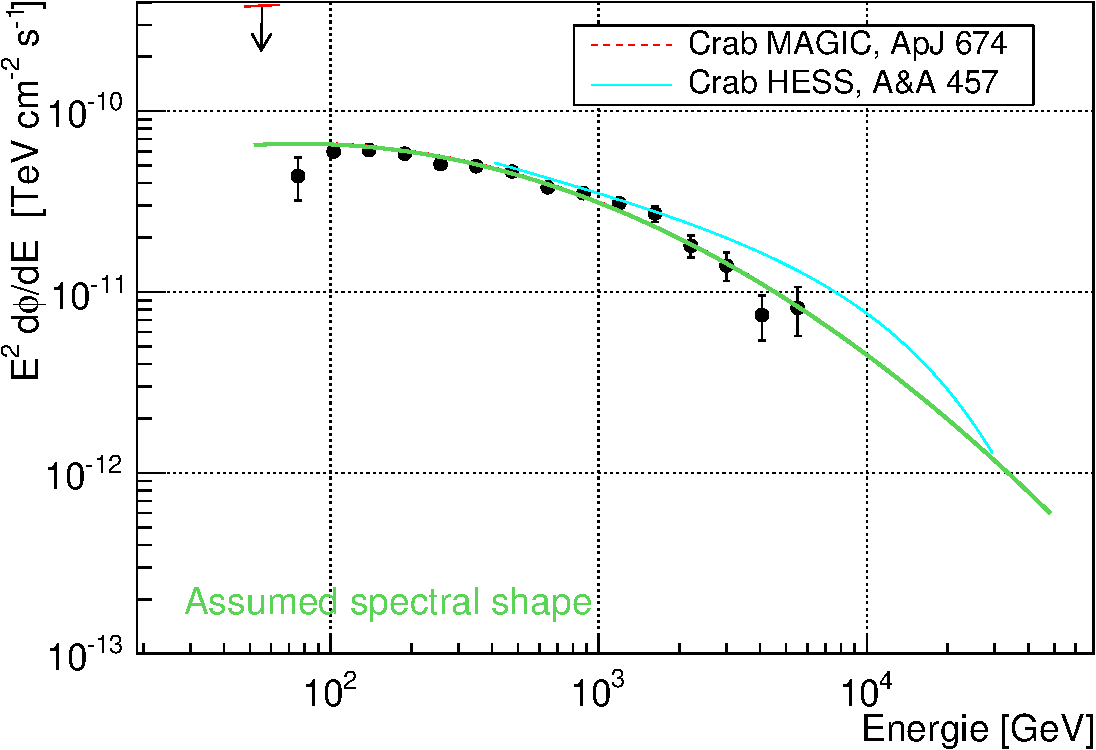
\includegraphics[width=\textwidth]{./Plots/04_MrkAnalyse/Datenset2/Crab_SED.pdf}
  \caption{Spektrale Energieverteilung}
  \label{Datenset2_SED_Crab}
  \end{subfigure}
  \hfill
  %-----------------------------Figure 4--------------------------------------------------------%
  \begin{subfigure}{0.45\linewidth}
  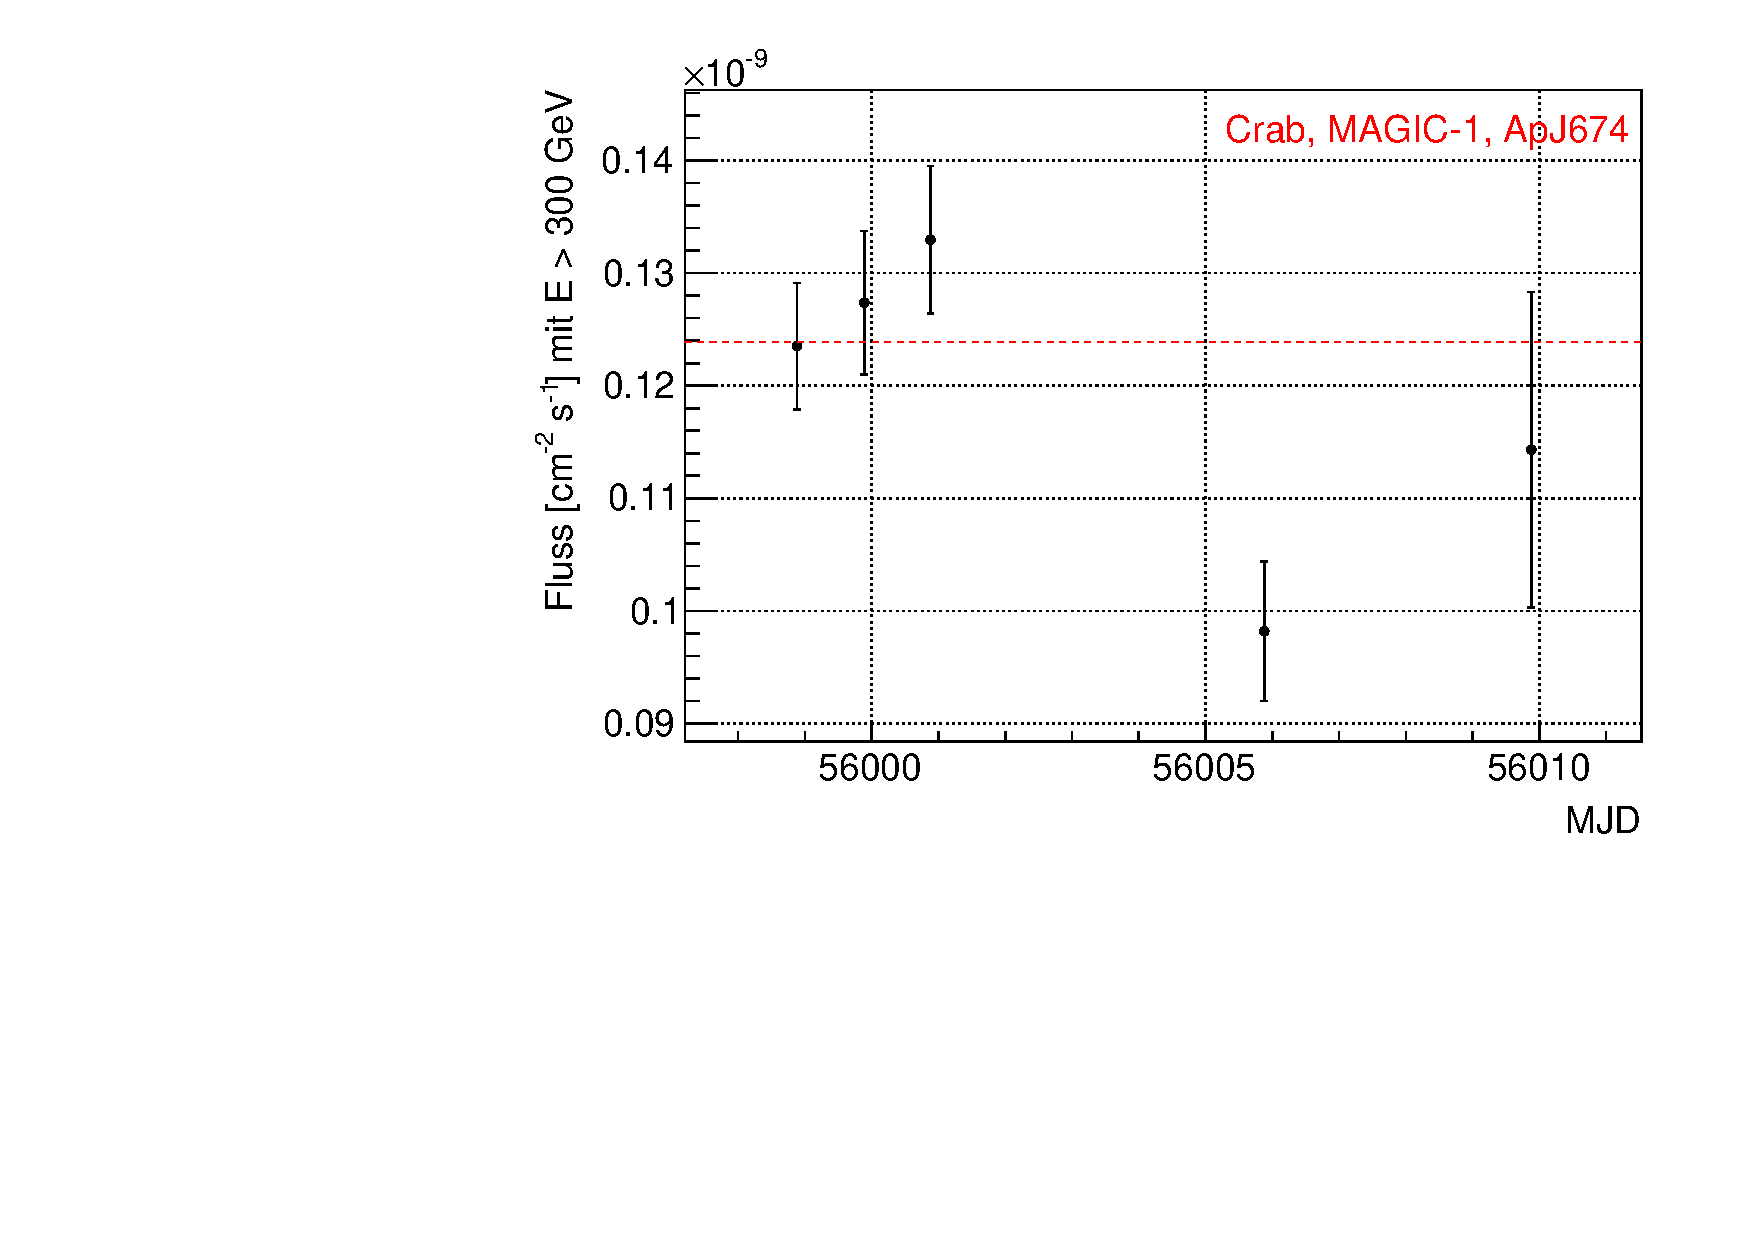
\includegraphics[width=\textwidth]{./Plots/04_MrkAnalyse/Datenset2/Crab_LC.pdf}
  \caption{Lichtkurve von Crab mit mittlerem Fluss von Crab, berechnet nach \cite{LiteraturreferenzMAGIC}.}
  \label{Datenset2_LC_Crab}
  \end{subfigure}
  \hfill
  %----------------------------------------------------------------------------------------------%
\caption{Genrierte Plots von \textit{Flute} für Crab-Daten}
\label{Datenset2_Flute_Plots_Crab}
\end{figure}

In \autoref{Datenset2_theta^2_Crab} ist der $\theta^2$-Plot für Crab zu sehen. Für kleine $\theta$ ist die Anzahl der Signal-Ereignisse ca. vier Mal höher als im Off-Bereich.

In \autoref{Datenset2_SpectralShape_Crab} ist das differentielle Energiespektrum zu sehen.

\autoref{Datenset2_SED_Crab} zeigt die spektrale Energieverteilung, d.h. das mit $E^2$ gewichtete Spektrum aus \autoref{Datenset2_SpectralShape_Crab}.
Das in der Literatur angegebene Spektrum ist durch eine rot gestrichelte Linie gekennzeichnet und wird von dem ermittelten Spektrum überdeckt, welches in grün dargestellt ist.

Wie in \autoref{Datenset2_SpectralShape_Crab} und in \autoref{Datenset2_SED_Crab} zu sehen, beschreibt das ermittelte Spektrum die Daten und ist konsistent mit dem bekannten Crab-Spektrum.
%Dieses angeonommene Spektrum ist in den beiden Abbildungen durch die grüne Linie gekennzeichnet.
Das ermittelte Spektrum folgt diesem Ausdruck:

\begin{equation}
\frac{\mathrm{d}N}{\mathrm{d}E} \propto \left(\frac{x}{\SI{300}{GeV}}\right)^{-2.31-0.26\cdot log_{10}(x/\SI{300}{GeV})}\si{TeV\,cm^{-2}\,s^{-1}}.
 %pow(x/300.,-2.31-0.26*log10(x/300.))
\end{equation}

Die Lichtkurve in Abb.\ref{Datenset2_LC_Crab} zeigt, dass der Crab-Fluss in diesem Zeitraum um den mittleren Crab-Fluss schwankt.
Die Parameter für den Hadroness-Schnitt bei 0,95 und den $\theta^2$-Schnitt bei 0,9, die zum Erstellen der Lichtkurve in \textit{Flute} verwendet wurden, können somit als korrekt angenommen werden.

\subsubsection{Lichtkurve: Mrk 421}
Es wird nun mit den gleichen Effizienz-Einstellungen wie für Crab eine Lichtkurve für Mrk 421 angefertigt.

\begin{figure}
    \centering
    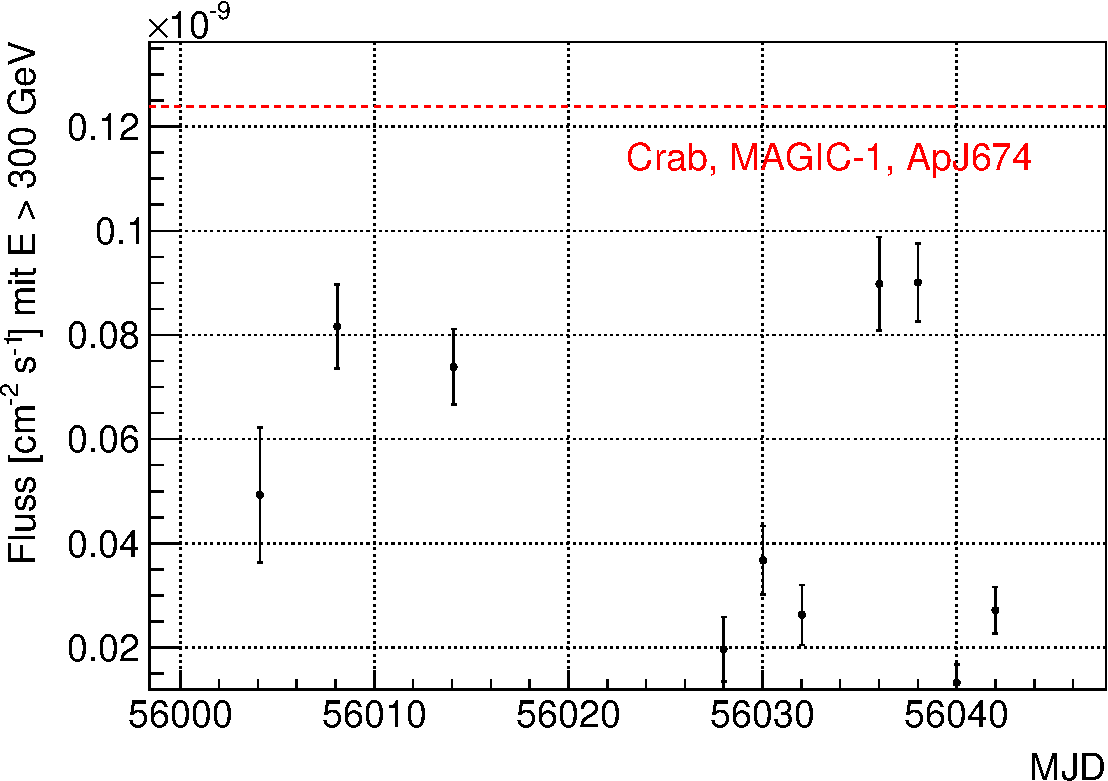
\includegraphics[width=0.8\textwidth]{./Plots/04_MrkAnalyse/Datenset2/LC_Mrk421.pdf}
    \caption{Lichtkurve von Mrk 421 im Zeitraum vom 18.3.2012 bis zum 25.4.2012.
    Der Fluss von Mrk~421 liegt im Durchschnitt bei 41\% des Flusses von Crab, den die rote Linie darstellt.}
    \label{Datenset2_LC_Mrk421}
\end{figure}

Die \autoref{Datenset2_LC_Mrk421} zeigt, dass der Fluss von Mrk 421 im Vergleich zu Crab niedriger ist.
Er schwankt etwa um den halben Crab-Fluss.
Auch die spektrale Energieverteilung unterscheidet sich von Crab (vgl. Abb.\ref{Datenset2_SED_Mrk421}), da ein anderes Spektrum angenommen wurde:

\begin{equation}
\frac{\mathrm{d}N}{\mathrm{d}E}\propto \left(\frac{x}{\SI{300}{GeV}}\right)^{-2.75}\si{TeV\,cm^{-2}\,s^{-1}}
\end{equation}


\begin{figure}
    \centering
    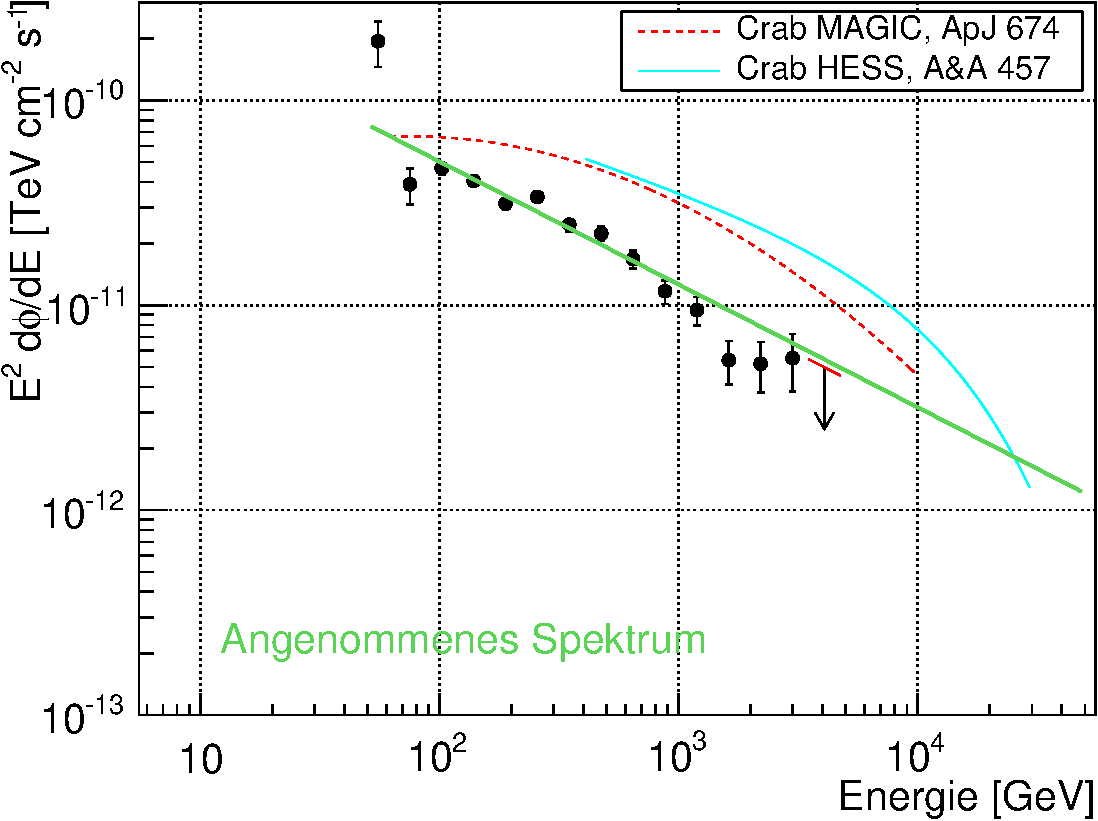
\includegraphics[width=0.8\textwidth]{./Plots/04_MrkAnalyse/Datenset2/SED_Mrk421.pdf}
    \caption{Spektrale Energieverteilung von Mrk 421.
    Zum Vergleich ist noch die spektrale Energieverteilung von Crab in rot eingezeichnet.}
    \label{Datenset2_SED_Mrk421}
\end{figure}


\subsubsection{Spektrum: Crab}
Mit Hilfe von \textit{CombUnfold} wird nun das Spektrum von Crab entfaltet.
In \autoref{Datenset2_CombunFold_Crab} ist das entfaltete Spektrum von Crab dargestellt, welches mit dem Literaturwert nach \cite{LiteraturreferenzMAGIC} berechnet wurde.

\begin{figure}
    \centering
    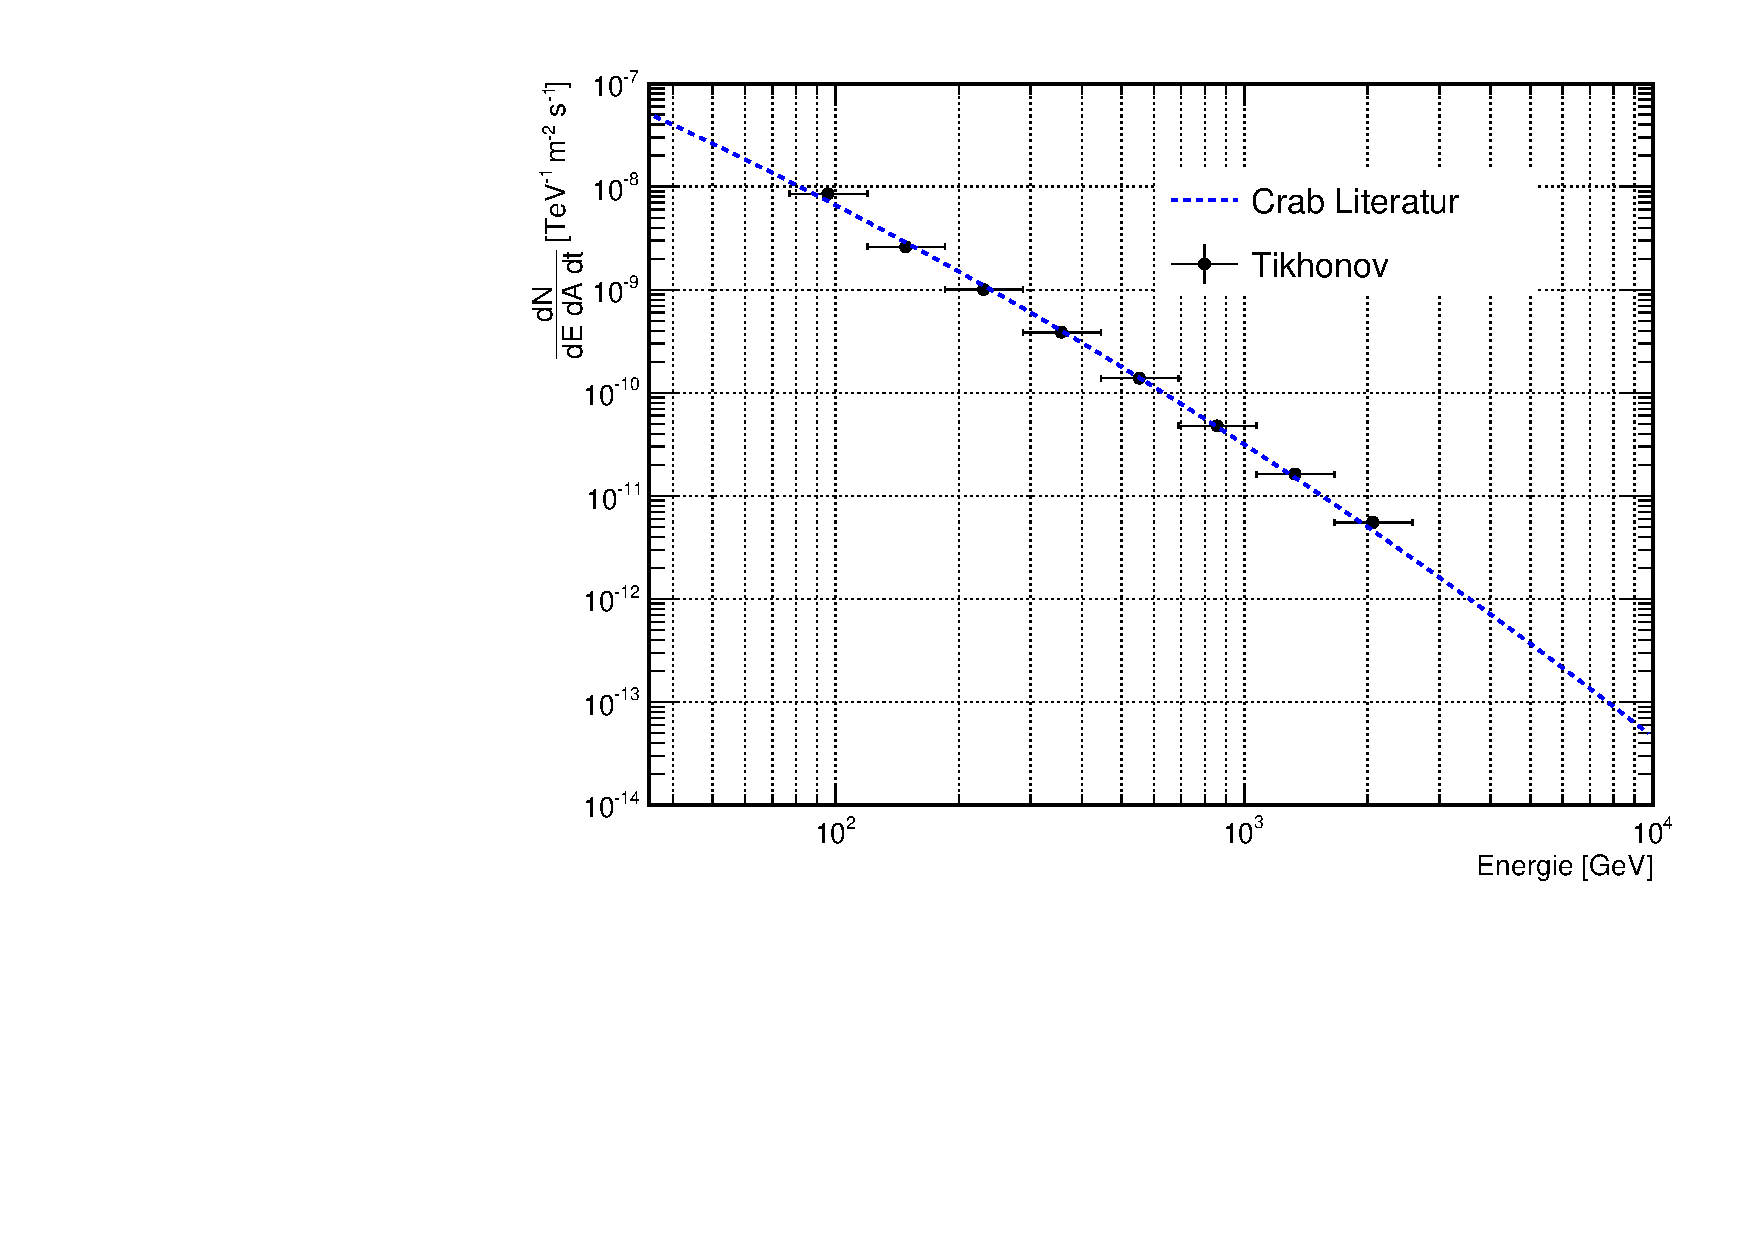
\includegraphics[width=0.8\textwidth]{./Plots/04_MrkAnalyse/Datenset2/Crab_mit_Literatur.pdf}
    \caption{Entfaltetes Crab-Spektrum im Zeitraum vom 18.3.2012 bis zum 25.4.2012 mit einem Literarurvergleich (siehe \cite{LiteraturreferenzMAGIC}).}
    \label{Datenset2_CombunFold_Crab}
\end{figure}

%Es zeigt sich, dass die entfalteten Datenpunkte mit Tikhonov-Regularisierung sehr gut zum Literaturwert passen.
Anhand dieser Entfaltung ist festzustellen, dass der ermittelte Fluss mit den bisherigen Messungen konsistent ist.

\subsubsection{Spektrum: Mrk 421}
Die \autoref{Datenset2_CombunFold_Mrk421} zeigt das entfaltete Spektrum von Mrk 421 mit fünf verschiedenen Regularisierungsmethoden.
Wie man sieht, zeigen die entfalteten Datenpunkte keine signifikanten Abweichungen voneinander. 
Lediglich bei kleinen Energien ist eine Anweichung zu erkennen, wleche allerdings weiterhin nicht signifikant ist.

\begin{figure}
    \centering
    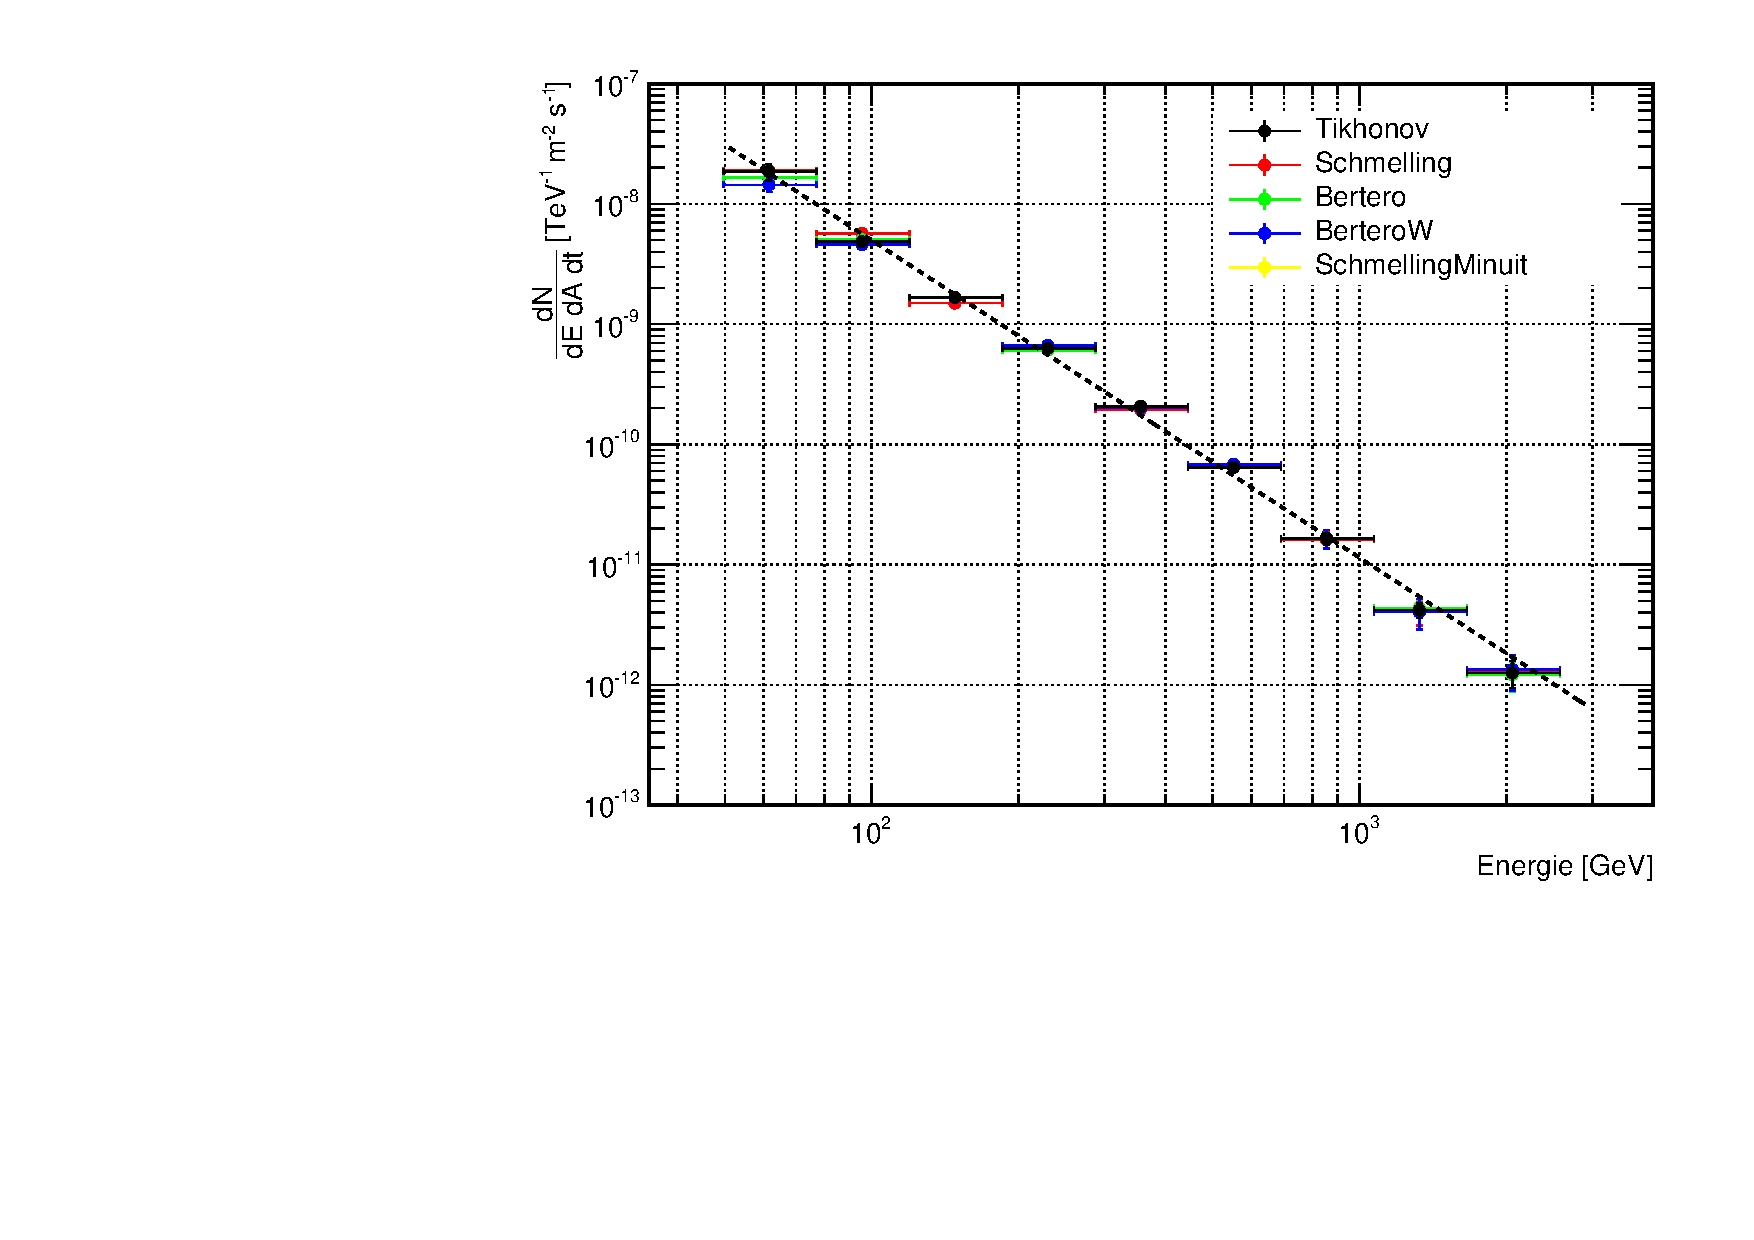
\includegraphics[width=0.8\textwidth]{./Plots/04_MrkAnalyse/Datenset2/Spektrum_Mrk421.pdf}
    \caption{Entfaltetes Mrk 421-Spektrum im Zeitraum vom 18.3.2012 bis zum 25.4.2012 mit allen wählbaren Regularisierungsmethoden.
    Die gestrichelte Linie stellt das gefittete Spektrum dar, welches mit Hilfe der Tikhonov-Regularisierung berechnet wurde.}
    \label{Datenset2_CombunFold_Mrk421}
\end{figure}

Es wurde zusätzlich der Fit dargestellt, der in der Entfaltung mit Tikhonov\-/Regularisierung erstellt wurde, da diese Regularisierungsmethode in den meisten Fällen die besten Ergebnisse lieferte.
Folgende Funktion wurde angenommen:

\begin{equation}
 \frac{\mathrm{d}N}{\mathrm{d}E\,\mathrm{d}A\,\mathrm{d}t}=f_0\left( \frac{E}{r} \right)^\alpha.
\end{equation}

Die angepasste Funktion ergibt sich somit zu:

\begin{equation}
 \frac{\mathrm{d}N}{\mathrm{d}E\,\mathrm{d}A\,\mathrm{d}t}=(2,74 \pm 0,06) \cdot 10^{-10}\left( \frac{E}{\SI{0,3}{TeV}} \right)^{-2.64 \pm 0,03} \si{TeV^{-1}\,s^{-1}\,cm^{-2}}.
\end{equation}


\FloatBarrier

\subsection{Datenset 1}
\label{subsec:Datenset_1}
Der folgende Teil beschreibt die Analyse der Daten vom 25.2.2012 und 29.2.2012.
Da diese Daten eine andere PSF haben als die Daten aus dem Datenset 2, benötigt es eigene MCs und die Daten müssen separat von Datenset 2 analysiert werden.
Die Daten an diesen zwei Tagen haben ebenfalls einen Zenitbereich von unter 35°.

\subsubsection{Datencheck}
Der Datencheck für diese Daten geschieht analog zum Datencheck des Datensets 2. 
Die Tabelle \ref{tab:Datenset1-Mrk421} zeigt an welchen Tagen Mrk 421-Daten den Datencheck überstanden haben und für die Analyse zur Verfügung stehen. 

\begin{table}[!h]
\centering
\caption{Übersicht über alle nach dem Datencheck zur Verfügung stehenden Daten von Mrk~421 aus Datenset 1.}
\label{tab:Datenset1-Mrk421}
\begin{tabular}{ll}
  \toprule
  Monat & Tage\\
  \midrule
  \midrule
Februar & 25., 29.\\
  \bottomrule
\end{tabular}
\end{table}


Tabelle \ref{tab:Datenset1} zeigt die selektierten Mrk 421-/Crab- und Background-Daten nach dem Datencheck.


\begin{table}[!h]
\centering
\caption{Übersicht über alle nach dem Datencheck zur Verfügung stehenden Daten von Mrk~421, Crab und Background aus Datenset 1.}
\label{tab:Datenset1}
\begin{tabular}{lc}
  \toprule
  Quelle & Obersvationszeit [min]\\
  \midrule
  \midrule
  Mrk 421 & 70\\
  \midrule
  Crab & 20\\
  \midrule
  0FGLJ0631 & 3 \\
  1ES1011 & 172 \\
  HB89 & 87 \\
  PG1553 & 115 \\
  PKS1222 & 106 \\
  SegueJ & 401 \\
  \bottomrule
  \bottomrule
\end{tabular}
\end{table}

\subsubsection{Lichtkurve: Crab und Mrk~421}
Mit Hilfe von Crab-Daten wurden die Einstellungen für die Lichtkurve von Mrk 421 bestimmt.
Es wurde nur an einem Tag zwischen dem 25.2.2012 und dem 29.2.2012 Crab beobachtet.
Deswegen beinhaltet die Lichtkurve von Crab nur $\SI{20}{min}$ an Crab-Daten (vgl. \autoref{Datenset1_LC_Crab}).

\begin{figure}
    \centering
    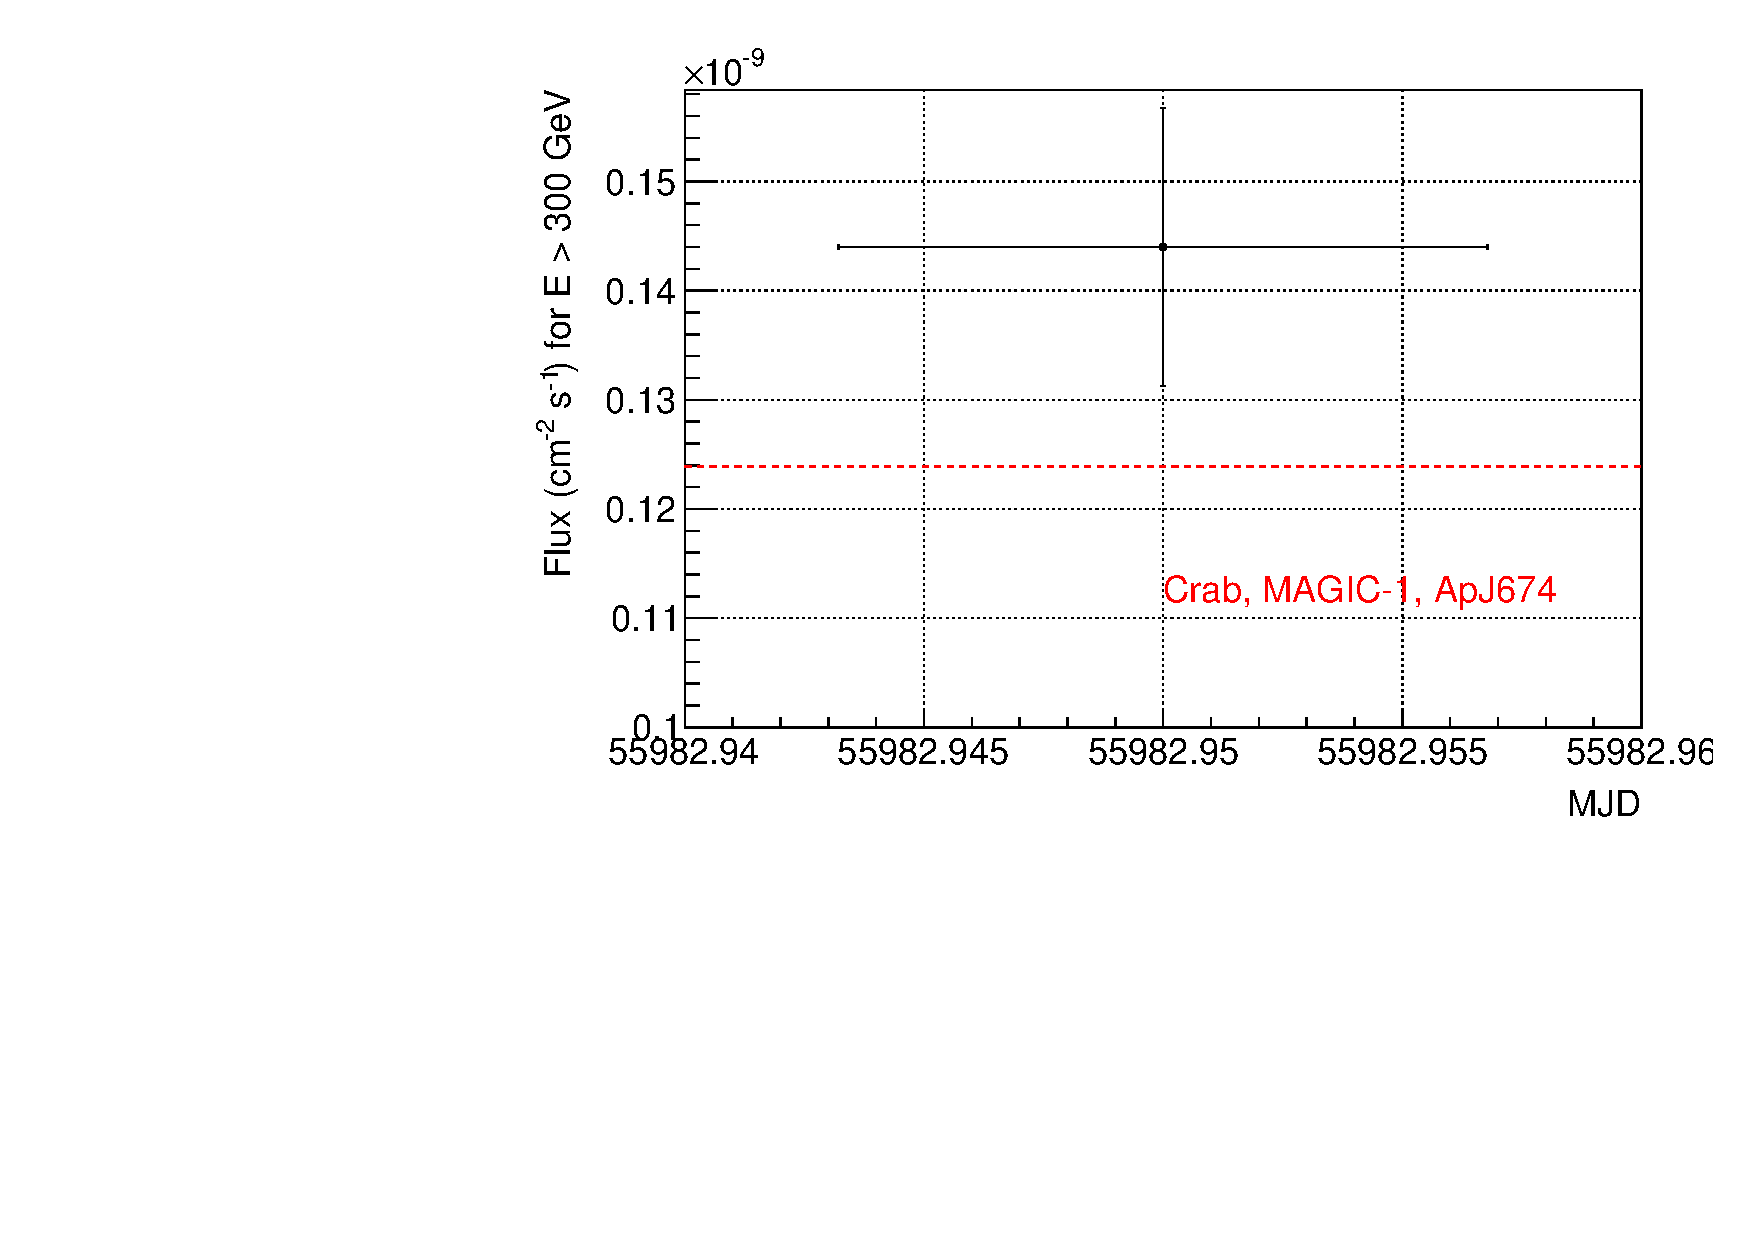
\includegraphics[width=0.8\textwidth]{./Plots/04_MrkAnalyse/Datenset1/Datenset1_LC_Crab.pdf}
    \caption{LC von Crab im Zeitraum vom 25.2.2012 bis zum 29.2.2012 mit dem mittleren Crab-Fluss (nach \cite{LiteraturreferenzMAGIC}).}
    \label{Datenset1_LC_Crab}
\end{figure}

Die Lichtkurve von Mrk 421 befindet sich in Abb.\ref{Datenset1_LC_Mrk421}.

\begin{figure}
    \centering
    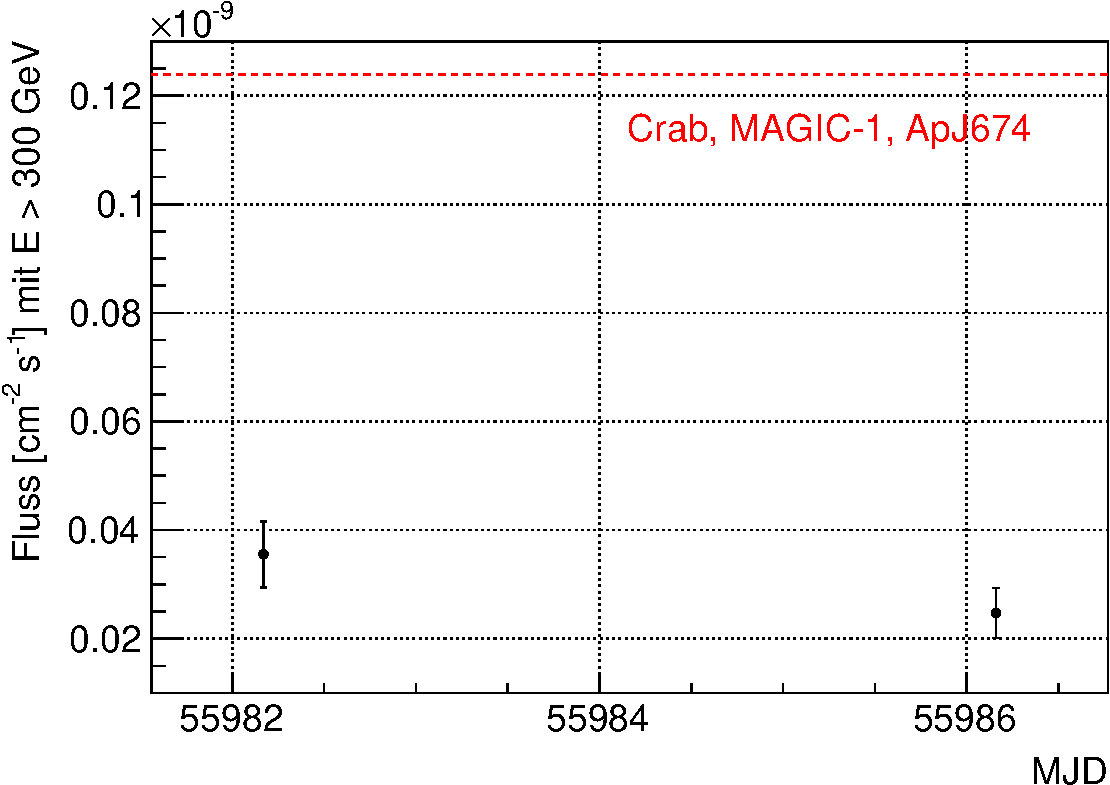
\includegraphics[width=0.8\textwidth]{./Plots/04_MrkAnalyse/Datenset1/Datenset1_LC_Mrk421.pdf}
    \caption{Lichtkurve von Mrk 421 im Zeitraum vom 25.2.2012 bis zum 29.2.2012.
    Der Fluss von Mrk~421 liegt im Durchschnitt bei 24\% des Flusses von Crab, den die rote Linie darstellt.}
    \label{Datenset1_LC_Mrk421}
\end{figure}

Es ist zu sehen, dass der Fluss an diesen beiden Tagen verglichen mit den Daten aus Datenset 2 auf einem niedrigen Niveau liegt.



\FloatBarrier

\subsubsection{Spektrum: Mrk~421}
Analog zu Datenset 2 wurde auch wieder ein Spektrum bestimmt.
Das Resultat befindet sich in Abb.\ref{Datenset1_Spektrum_Mrk421}.

\begin{figure}
    \centering
    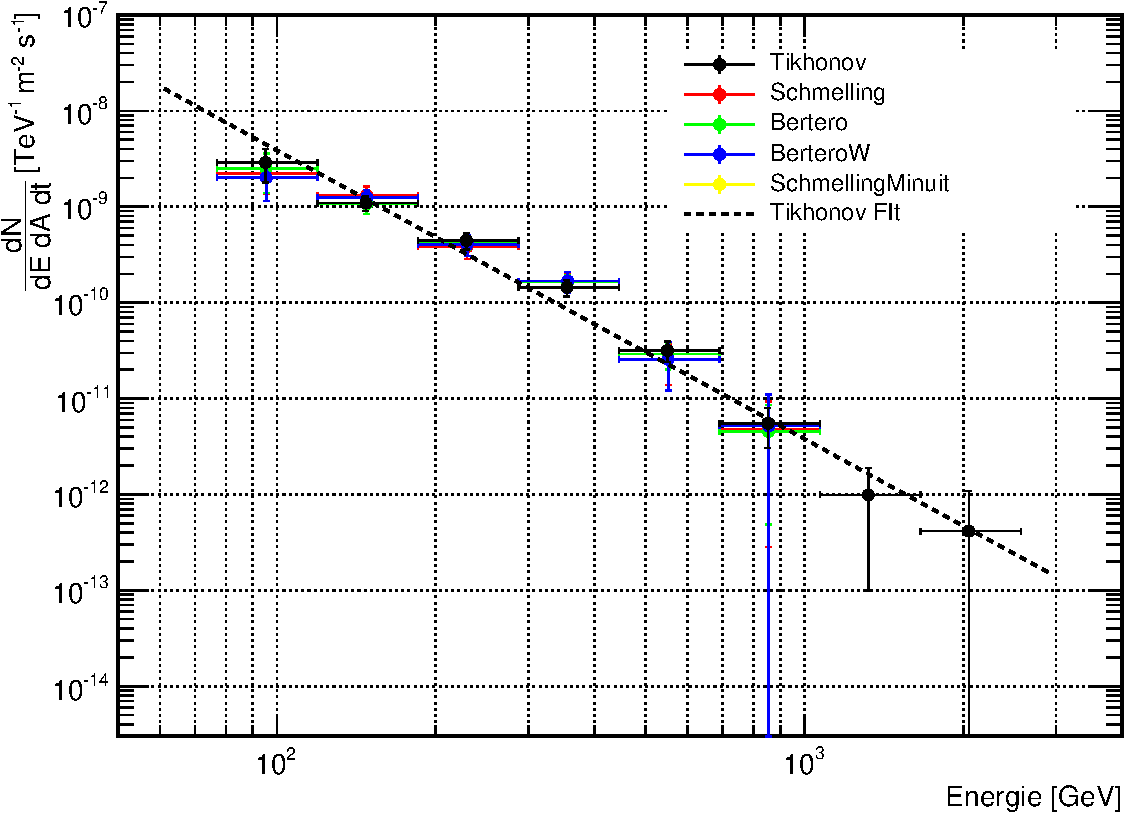
\includegraphics[width=0.8\textwidth]{./Plots/04_MrkAnalyse/Datenset1/Spektrum_Mrk421.pdf}
    \caption{Entfaltetes Spektrum von Mrk 421 im Zeitraum vom 25.2.2012 bis zum 29.2.2012 mit allen wählbaren Regularisierungsmethoden.
    Die gestrichelte Linie stellt das gefittete Spektrum dar, welches mit Hilfe der Tikhonov-Regularisierung berechnet wurde.}
    \label{Datenset1_Spektrum_Mrk421}
\end{figure}

Es ist zu sehen, dass die Entfaltungen ohne Tikhonov-Regularisierung im hohen Energiebereich, d.h $E>\SI{9}{TeV}$, keine Ergebnisse liefern .
Aufgrund des großen Energiebereichs, in dem die Entfaltung mit Tikhonov-Regularisierung Ergebnisse liefert, wird wieder dieser Fit der Daten eingezeichnet.
Der Fit lieferte folgendes Ergebnis:

\begin{equation}
 \frac{\mathrm{d}N}{\mathrm{d}E\mathrm{d}A\mathrm{d}t}=(1,42 \pm 0,11) \cdot 10^{-11}\left( \frac{E}{0,3 \si{TeV}} \right)^{-3.01\pm 0,14} \si{TeV^{-1}\,s^{-1}\,cm^{-2}}.
\end{equation}

Aufgrund der kurzen Observationszeit wurde keine Entfaltung der Crab-Daten vorgenommen.

\FloatBarrier

\subsection{Datenset 4}
\label{subsec:Datenset_4}
Dieses Datenset beinhaltet die ersten Daten, die von Mrk 421 nach dem Austausch der MAGIC-I-Kamera aufgenommen wurden. 
Wie das Datenset 1 umfasst dieses Datenset nur wenige Tage. 
An drei Tagen wurde Mrk~421 im Stereo-Modus observiert. 

\subsubsection{Datencheck}
Der Datencheck für diese Daten geschieht analog zum Datencheck des Datensets 2. 
Die \autoref{tab:Datenset4} zeigt, welche Mrk 421-/Crab- und Background-Daten nach dem Datencheck vorhanden sind und die \autoref{tab:Datenset4-Mrk421} zeigt, an welchen Tage die Mrk 421-Daten genommen wurden.

\begin{table}[!h]
\centering
\caption{Übersicht über alle an nach dem Datencheck zur Verfügung stehenden Daten von Mrk~421 aus Datenset 4.}
\label{tab:Datenset4-Mrk421}
\begin{tabular}{ll}
  \toprule
  Monat & Tage\\
  \midrule
  \midrule
Dezember & 15., 19., 23.\\
  \bottomrule
\end{tabular}
\end{table}


\begin{table}[!h]
\centering
\caption{Übersicht über alle an nach dem Datencheck zur Verfügung stehenden Daten von Mrk~421, Crab und Background aus Datenset 4.}
\label{tab:Datenset4}
\begin{tabular}{lc}
  \toprule
  Quelle & Observationszeit [min]\\
  \midrule
  \midrule
  Mrk 421 & 74\\
  \midrule
  Crab & 852\\
  \midrule
  1ES0229 & 221 \\
  NGC1275 & 112 \\
  SegueA & 900  \\
  \bottomrule
  \bottomrule
\end{tabular}
\end{table}

\subsubsection{Lichtkurve: Crab und Mrk~421}
Die Lichtkurve von Crab befindet sich in \autoref{Datenset4_LC_Crab}. 
Es ist zu sehen, dass diese Lichtkurve mit dem mittleren Fluss von Crab gut übereinstimmt.
Die Lichtkurve von Mrk 421 ist in \autoref{Datenset4_LC_Mrk421}. 
In diesem Zeitraum liegt der Mrk~412-Fluss weiterhin unterhalb des Crab-Flusses.

\begin{figure}
    \centering
    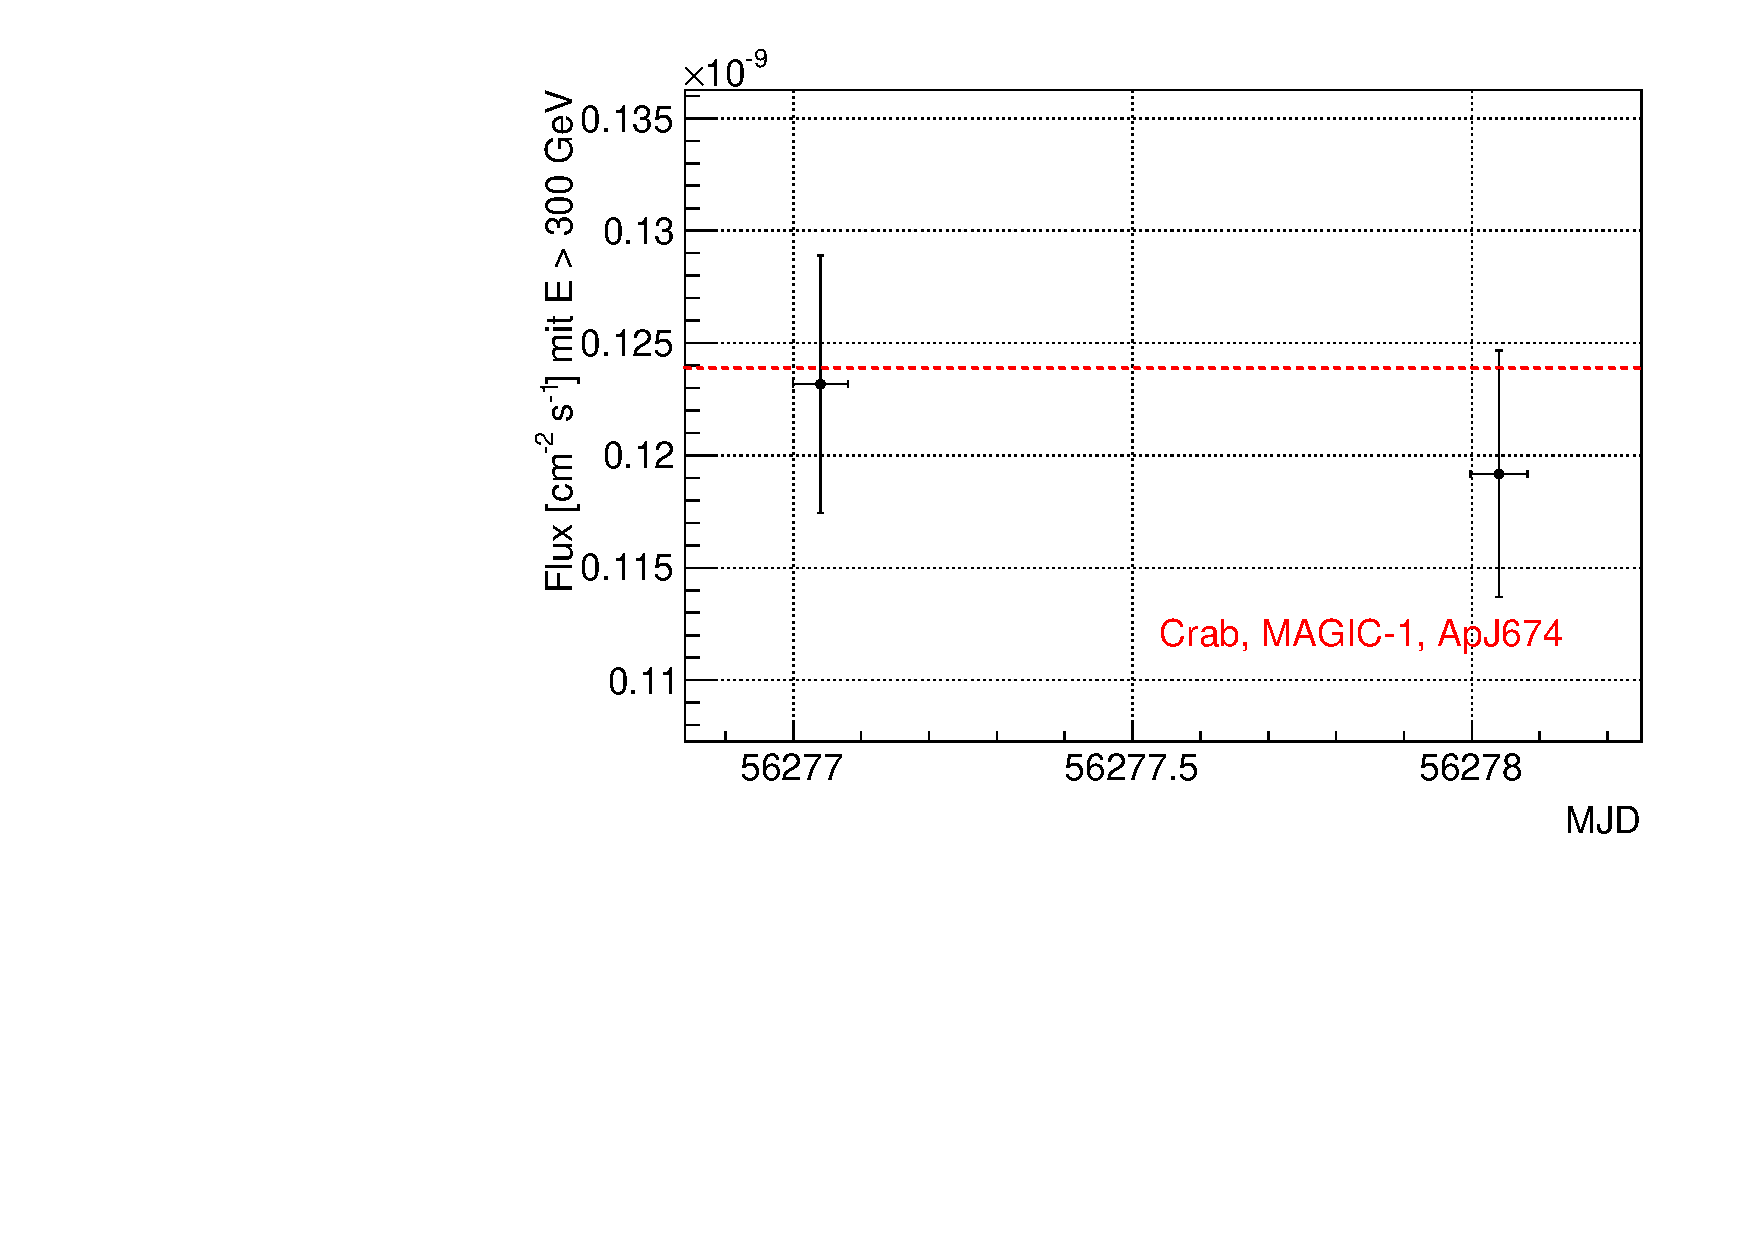
\includegraphics[width=0.8\textwidth]{./Plots/04_MrkAnalyse/Datenset4/Datenset4_LC_Crab.pdf}
    \caption{Lichtkurve Crab im Zeitraum vom 15.12.2012 bis zum 23.12.2012.
    Die Werte liegen nah am mittleren Fluss von Crab, welcher mit \cite{LiteraturreferenzMAGIC} berechnet wurde.}
    \label{Datenset4_LC_Crab}
\end{figure}

\begin{figure}
    \centering
    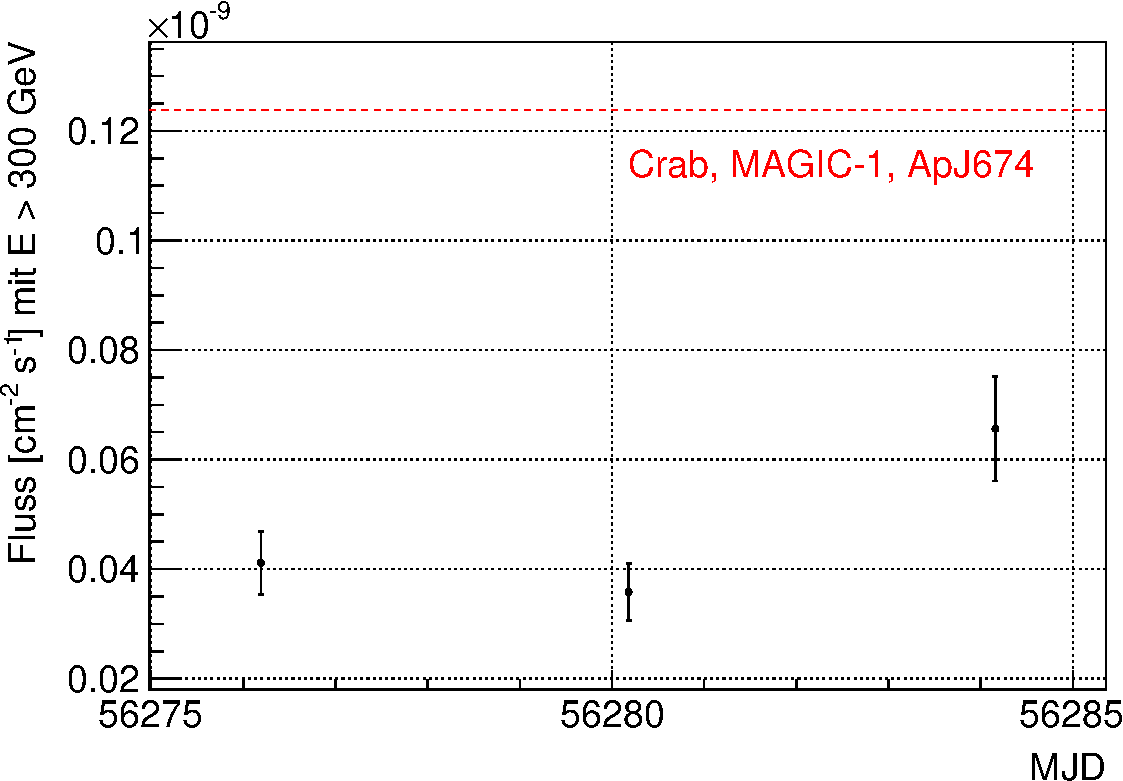
\includegraphics[width=0.8\textwidth]{./Plots/04_MrkAnalyse/Datenset4/Datenset4_LC_Mrk421.pdf}
    \caption{Lichtkurve Mrk 421 im Zeitraum vom 15.12.2012 bis zum 23.12.2012.
    Der Fluss von Mrk~421 liegt im Durchschnitt bei 38\% des Flusses von Crab, den die rote Linie darstellt.}
    \label{Datenset4_LC_Mrk421}
\end{figure}


\subsubsection{Spektrum: Mrk~421}
Das entfaltete Spektrum von Mrk 421 befindet sich in Abb.~\ref{Datenset4_Spektrum_Mrk421}.

\begin{figure}
    \centering
    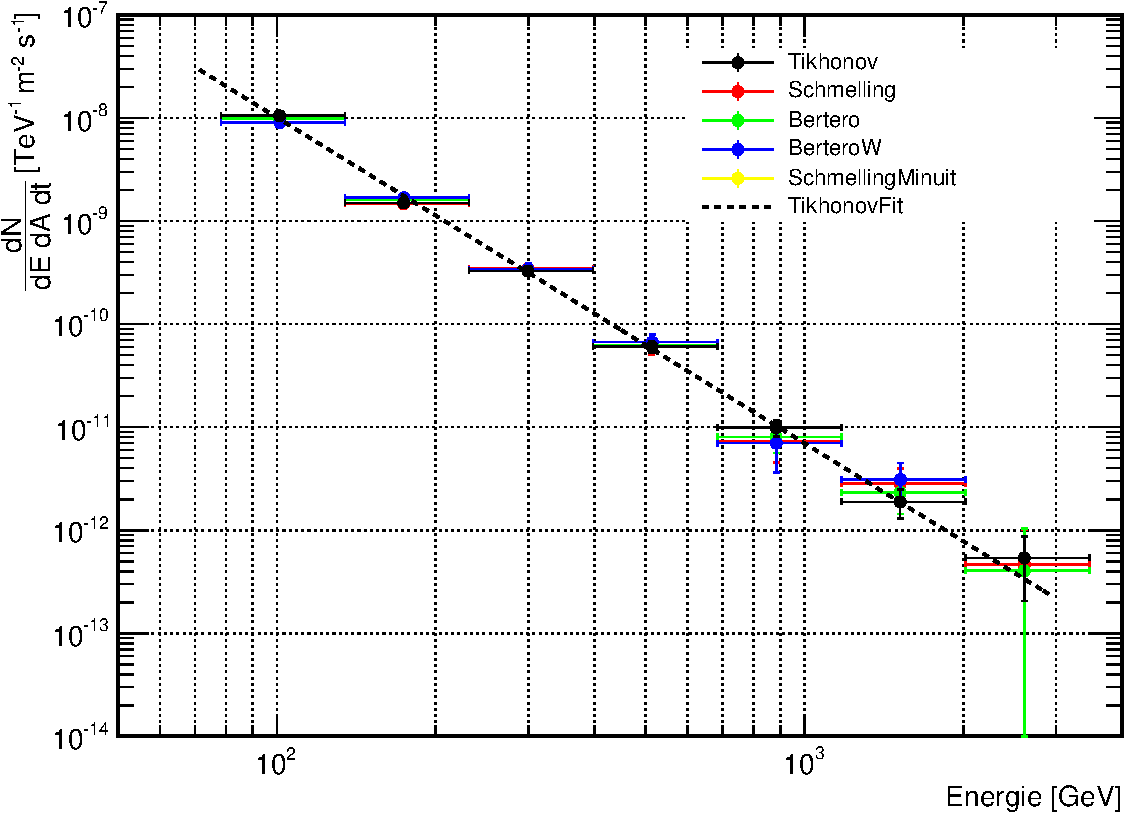
\includegraphics[width=0.8\textwidth]{./Plots/04_MrkAnalyse/Datenset4/Datenset4_Spektrum_Mrk421.pdf}
    \caption{Entfaltetes Spektrum von Mrk 421 im Zeitraum vom 15.12.2012 bis zum 23.12.2012 mit allen wählbaren Regularisierungsmethoden.
    Die gestrichelte Linie stellt das gefittete Spektrum dar, welches mit Hilfe der Tikhonov-Regularisierung berechnet wurde.}
    \label{Datenset4_Spektrum_Mrk421}
\end{figure}

Der Fit des entfalteten Spektrums mit Tikhonov-Regularisierung liefert folgendes Ergebnis:

\begin{equation}
 \frac{\mathrm{d}N}{\mathrm{d}E\mathrm{d}A\mathrm{d}t}=(3,14 \pm 0,15) \cdot 10^{-10}\left( \frac{E}{0,3 \si{TeV}} \right)^{-3.16\pm 0,07} \si{TeV^{-1}\,s^{-1}\,cm^{-2}}.
\end{equation}


\FloatBarrier

\subsection{Datenset 3}
\label{subsec:Datenset_3}

\subsubsection{Datencheck}
Der Datencheck für die Mono-Daten geschieht analog zum Datencheck der anderen Datensets.
Die Analyse beruht auf Daten auf Star-Level und nicht Superstar-Level wie zuvor.
Tabelle \ref{tab:Datenset3-Mrk421} und Tabelle \ref{tab:Datenset3} zeigen, welche Mrk 421-und Background-Daten nach dem Datencheck vorhanden sind.
Ein Beobachtung von Crab find in diesem Zeitraum nicht statt.

\begin{table}[!h]
\centering
\caption{Übersicht über alle nach dem Datencheck zur Verfügung stehenden Daten von Mrk~421 aus Datenset 3.}
\label{tab:Datenset3-Mrk421}
\begin{tabular}{ll}
  \toprule
  Monat & Tage\\
  \midrule
  \midrule
Mai & 23., 25., 26., 27.\\
Juni & 15,. 19. \\
  \bottomrule
\end{tabular}
\end{table}


\begin{table}[!h]
\centering
\caption{Übersicht über alle nach dem Datencheck zur Verfügung stehenden Daten von Mrk~421, Crab und Background aus Datenset 3}
\label{tab:Datenset3}
\begin{tabular}{lc}
  \toprule
  Quelle & Observationszeit [min]\\
  \midrule
  \midrule
  Mrk 421 & 333\\
  \midrule
  1ES1959 & 360 \\
  AE-Aqr & 54  \\
  HD215227 & 649 \\
  M87 & 64 \\
  \bottomrule
  \bottomrule
\end{tabular}
\end{table}

\subsubsection{Energieschätzung}
Im Vergleich zu der Stereo-Analyse müssen für die Mono-Analyse ältere Programme verwendet werden.
Die RFs für die \texttt{Disp}-Bestimmung und Gamma-Hadron-Separation werden mit Hilfe von \textit{Osteria} erstellt.
Im Gegensatz zur Standardanalyse werden keine Look-Up-Tables zur Energieschätzung benutzt, sondern ebenfalls ein RF.

\subsubsection{Lichtkurve: Mrk~421}
Nachdem allen Ereignissen eine Hadroness, ein \texttt{Disp}-Wert sowie eine geschätzte Energie zugeordnet worden sind, wird nach Anwendung eines Hadroness-Schnittes eine Lichtkurve erstellt.
Dies geschieht mit Hilfe des Programms \textit{Fluxlc}.
Obwohl keine Crab-Daten zur Verfügung standen, um die Einstellungen für die Lichtkurve mit einem bekannten Fluss zu überprüfen, wird eine Lichtkurve für Mrk 421 erstellt.
\autoref{Datenset3_LC_Mrk421} zeigt die Lichtkurve für Mrk 421.

\begin{figure}
    \centering
    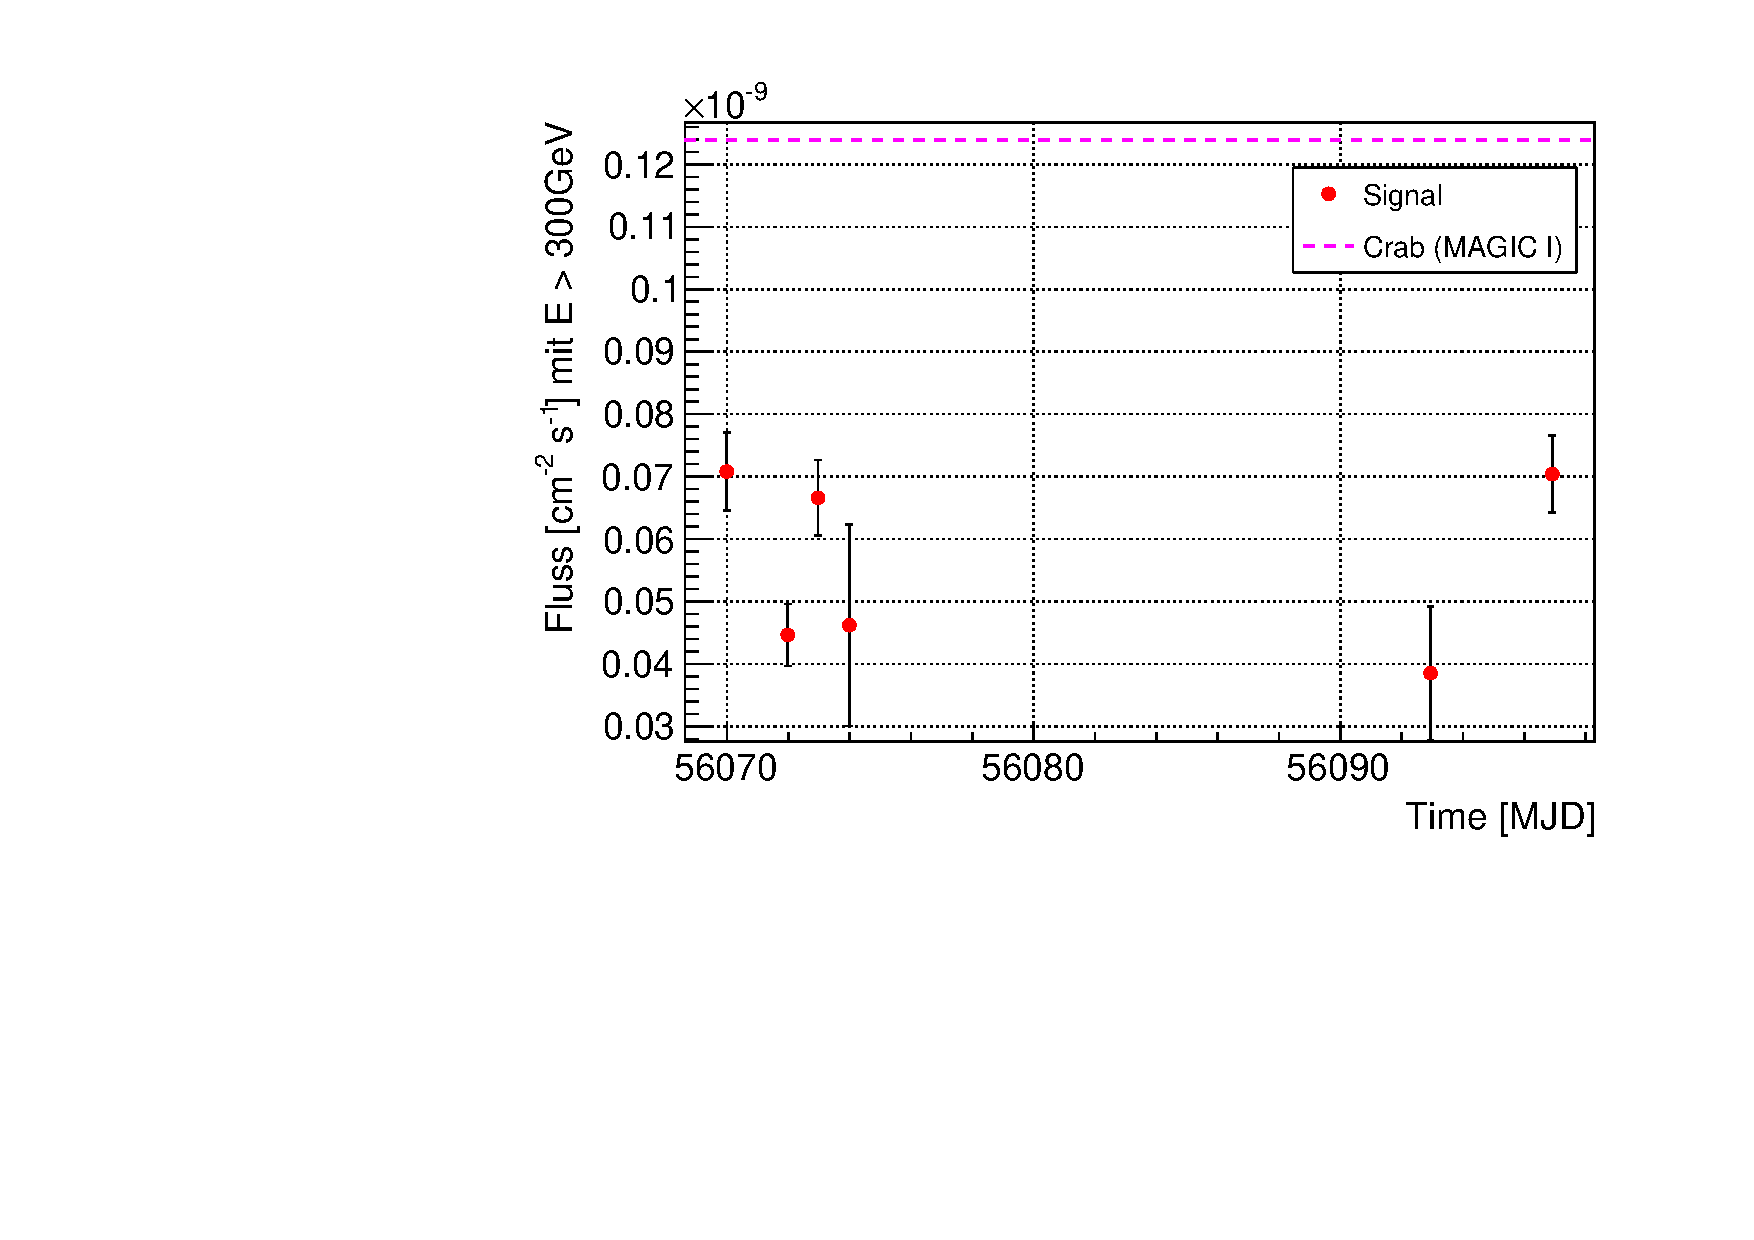
\includegraphics[width=0.8\textwidth]{./Plots/04_MrkAnalyse/Datenset3/Datenset3_Mrk421_LC.pdf}
    \caption{Lichtkurve von Mrk 421 im Zeitraum vom 23.05.2012 bis zum 19.05.2012.
    Der Fluss von Mrk~421 liegt im Durchschnitt bei 45\% des Flusses von Crab, den die rosane Linie darstellt.}
    \label{Datenset3_LC_Mrk421}
\end{figure}

Es zeigt sich, dass der Fluss von Mrk 421 in diesem Zeitbereich genau wie in den anderen Zeitbereichen ebenfalls geringer als der Crab-Fluss ist.


\subsubsection{Spektrum}

In \autoref{Datenset3_Spektrum_Mrk421} ist das entfaltete Spektrum für diesen Zeitraum dargestellt.
Der Fit an die Datenpunkte nach der Entfaltung mit Tikhonov-Regularisierung liefert folgendes Ergebnis:

\begin{equation}
 \frac{\mathrm{d}N}{\mathrm{d}E\mathrm{d}A\mathrm{d}t}=(5,42 \pm 0.23) \cdot 10^{-10}\left( \frac{E}{\SI{0,3}{TeV}} \right)^{(-3.25 \pm 0.09)} \si{TeV^{-1}\,s^{-1}\,cm^{-2}}.
\end{equation}

\begin{figure}
    \centering
    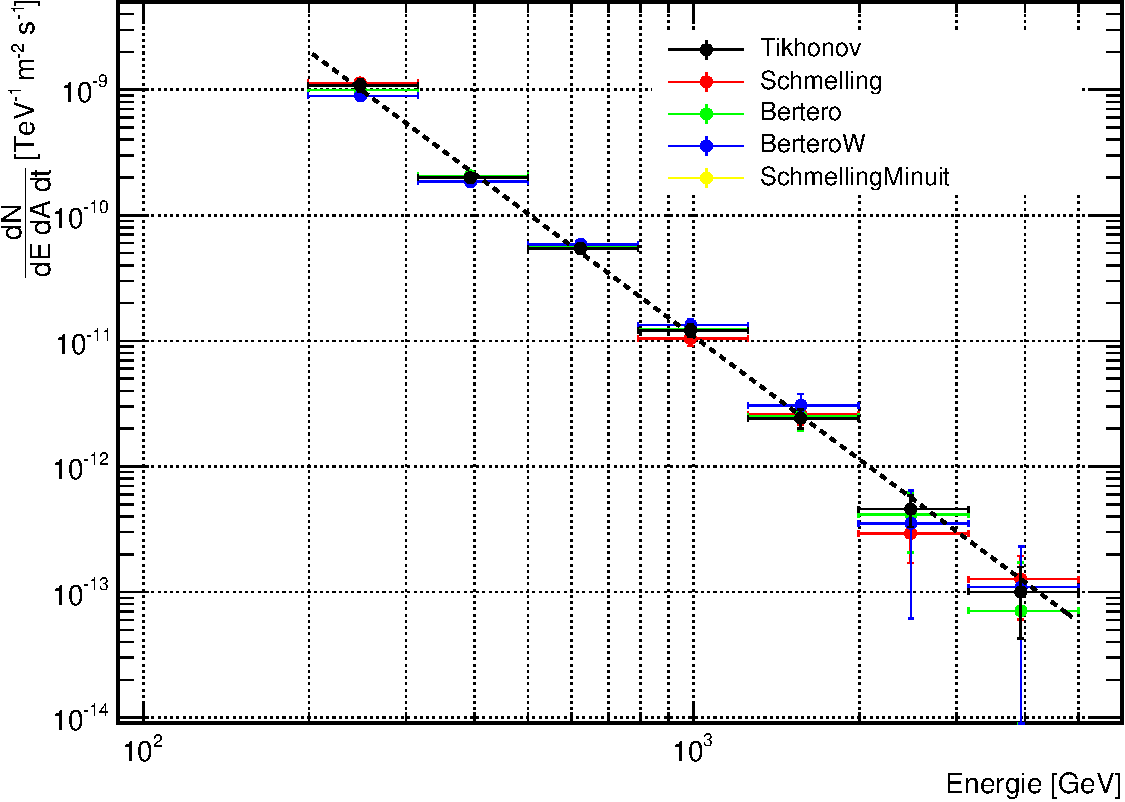
\includegraphics[width=0.8\textwidth]{./Plots/04_MrkAnalyse/Datenset3/Datenset3_Mrk421_Spektrum.pdf}
    \caption{Spektrum von Mrk 421 im Zeitraum vom 23.05.2012 bis zum 19.06.2012 mit allen wählbaren Regularisierungsmethoden.
    Die gestrichelte Linie stellt das gefittete Spektrum dar, welches mit Hilfe der Tikhonov-Regularisierung berechnet wurde.}
    \label{Datenset3_Spektrum_Mrk421}
\end{figure}

\FloatBarrier


\section{Zusammenfassung der Ergebnisse und Vergleich der Datensets}
\label{LC_Alles}

Nachdem für jedes Datenset einzelne Lichtkurven erstellt worden sind, sind in \autoref{Alles_LC_Mrk421} nun alle Daten in einer Lichtkurve dargestellt.
Da zwischen dem 20.06.2012 und dem 10.12.2012 keine Daten von Mrk 421 genommen wurden, weil die MAGIC-I-Kamera außer Betrieb war, das Upgrade durchgeführt wurde und Mrk~421 zwischen Juli und November nicht beobachtbar ist, befindet sich eine Lücke in der Lichtkurve.

\begin{figure}
    \centering
    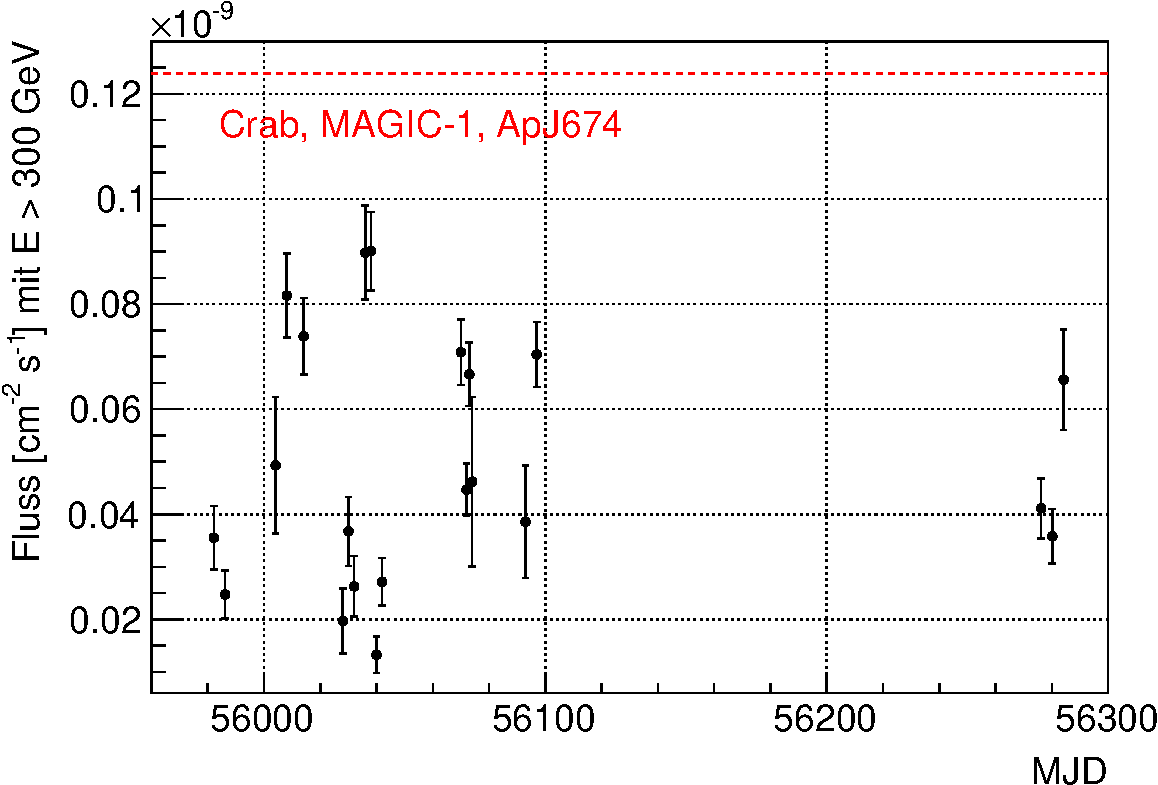
\includegraphics[width=0.8\textwidth]{./Plots/04_MrkAnalyse/Alles_LC.pdf}
    \caption{Zusammenfassende Lichtkurve der Mrk~421-Daten.
    Es sind alle vorher berechneten Lichtkurven-Daten in einem Diagramm dargestellt. 
    Es ist zu sehen, dass der Fluss von Mrk~421 im gesamten Jahr 2012 unterhalb des mittleren Flusses von Crab liegt, allerdings durchaus zeitliche Variabilitäten aufweist, die nachfolgend untersucht wird.}
    \label{Alles_LC_Mrk421}
\end{figure}

Anhand der Abbildung ist zu sehen, dass alle Datenpunkte etwa auf dem gleichen niedrigen Niveau liegen.
Der Fluss von Crab wird zu keinem Zeitpunkt erreicht.
Physikalisch interessante Phänomene wie Flares wurden im gesamten Jahr 2012 von MAGIC nicht beobachtet.
%Im April 2013 trat beispielsweise ein Flare auf.
Verglichen mit dem gesamten Fluss von MAGIC zwischen Dezember 2004 und Dezember 2009 \cite{DissBackes} ist der Fluss von 2012 auf einem niedrigen Niveau.
Im Dezember 2006 war er an vielen Tagen auf einem ähnlich niedrigen Niveau.

Im Gegensatz zu den Flares von 2007 und 2008, bei denen der Fluss bis zu 20 mal so hoch wie zu ruhigen Zeiten \cite{DissBackes}  war, ist der Fluss 2012 konstant niedrig.

Ein Vergleich mit dem Fluss zwischen Januar und Mai 2009 \cite{DissDiego} liefert ebenfalls das Ergebnis, dass sich Mrk 421 2012 in einem ruhigen Zustand befand.

In \autoref{tab:SpektraleIndizes} sind die spektralen Indizes der Entfaltung der einzelnen Datensets zusammengefasst.
Die spektralen Indizes der Datensets 1,3 und 4 beschreiben ein steiles Spektrum mit relativ niedrigem hochenergetischem Fluss.
Datenset 2 hat einen kleineren spektralen Index, d.h. das Spektrum ist härter, wobei der Fluss wie oben erwähnt, den Crab-Fluss nicht erreicht.


\begin{table}[!h]
\centering
\caption{Vergleich der spektralen Indizes und Flusskonstanten der einzelnen Datensets.}
\label{tab:SpektraleIndizes}
\begin{tabular}{lll}
  \toprule
  Datenset & Normierung $\left[\si{TeV^{-1}\,cm^{-2}\,s^{-1}}\right]$ & spektraler Index\\
  \midrule
  \midrule
Datenset 1 & $(1,42\pm 0,11)\cdot 10^{-10}$ & -3,01 $\pm$ 0,14 \\
Datenset 2 & $(2,74\pm 0,06)\cdot 10^{-10}$ & -2,64 $\pm$ 0,03 \\
Datenset 3 & $(5,42\pm 0,23)\cdot 10^{-10}$ & -3,25 $\pm$ 0,09 \\
Datenset 4 & $(3,14\pm 0,15)\cdot 10^{-10}$ & -3,16 $\pm$ 0,07 \\
  \bottomrule
\end{tabular}
\end{table}

